%%%%%%%%%%%%%%
%% Run LaTeX on this file several times to get Table of Contents,
%% cross-references, and citations.

%% If you have font problems, you may edit the w-bookps.sty file
%% to customize the font names to match those on your system.

%% w-bksamp.tex. Current Version: Feb 16, 2012
%%%%%%%%%%%%%%%%%%%%%%%%%%%%%%%%%%%%%%%%%%%%%%%%%%%%%%%%%%%%%%%%
%
%  Sample file for
%  Wiley Book Style, Design No.: SD 001B, 7x10
%  Wiley Book Style, Design No.: SD 004B, 6x9
%
%
%  Prepared by Amy Hendrickson, TeXnology Inc.
%  http://www.texnology.com
%%%%%%%%%%%%%%%%%%%%%%%%%%%%%%%%%%%%%%%%%%%%%%%%%%%%%%%%%%%%%%%%

%%%%%%%%%%%%%
% 7x10
%\documentclass{wileySev}

% 6x9
\documentclass{wileySix}

\usepackage{graphicx}

%%%%%%%
%% for times math: However, this package disables bold math (!)
%% \mathbf{x} will still work, but you will not have bold math
%% in section heads or chapter titles. If you don't use math
%% in those environments, mathptmx might be a good choice.

% \usepackage{mathptmx}

% For PostScript text
\usepackage{w-bookps}

%%%%%%%%%%%%%%%%%%%%%%%%%%%%%%%%%%%%%%%%%%%%%%%%%%%%%%%%%%%%%%%%
%% Other packages you might want to use:

% for chapter bibliography made with BibTeX
% \usepackage{chapterbib}

% for multiple indices
% \usepackage{multind}

% for answers to problems
% \usepackage{answers}

%%%%%%%%%%%%%%%%%%%%%%%%%%%%%%
%% Change options here if you want:
%%
%% How many levels of section head would you like numbered?
%% 0= no section numbers, 1= section, 2= subsection, 3= subsubsection
%%==>>
\setcounter{secnumdepth}{3}

%% How many levels of section head would you like to appear in the
%% Table of Contents?
%% 0= chapter titles, 1= section titles, 2= subsection titles, 
%% 3= subsubsection titles.
%%==>>
\setcounter{tocdepth}{2}

%% Cropmarks? good for final page makeup
%% \docropmarks

%%%%%%%%%%%%%%%%%%%%%%%%%%%%%%
%
% DRAFT
%
% Uncomment to get double spacing between lines, current date and time
% printed at bottom of page.
% \draft
% (If you want to keep tables from becoming double spaced also uncomment
% this):
% \renewcommand{\arraystretch}{0.6}
%%%%%%%%%%%%%%%%%%%%%%%%%%%%%%

%%%%%%% Demo of section head containing sample macro:
%% To get a macro to expand correctly in a section head, with upper and
%% lower case math, put the definition and set the box 
%% before \begin{document}, so that when it appears in the 
%% table of contents it will also work:

\newcommand{\VT}[1]{\ensuremath{{V_{T#1}}}}

%% use a box to expand the macro before we put it into the section head:

\newbox\sectsavebox
\setbox\sectsavebox=\hbox{\boldmath\VT{xyz}}

%%%%%%%%%%%%%%%%% End Demo


\begin{document}


\booktitle{Survey Methodology}
\subtitle{This is the Subtitle}

\authors{Robert M. Groves\\
\affil{Universitat de les Illes Balears}
Floyd J. Fowler, Jr.\\
\affil{University of New Mexico}
}

\offprintinfo{Survey Methodology, Second Edition}{Robert M. Groves}

%% Can use \\ if title, and edition are too wide, ie,
%% \offprintinfo{Survey Methodology,\\ Second Edition}{Robert M. Groves}

%%%%%%%%%%%%%%%%%%%%%%%%%%%%%%
%% 
\halftitlepage

\titlepage


\begin{copyrightpage}{2007}
Survey Methodology / Robert M. Groves . . . [et al.].
\       p. cm.---(Wiley series in survey methodology)
\    ``Wiley-Interscience."
\    Includes bibliographical references and index.
\    ISBN 0-471-48348-6 (pbk.)
\    1. Surveys---Methodology.  2. Social 
\  sciences---Research---Statistical methods.  I. Groves, Robert M.  II. %
Series.\\

HA31.2.S873 2007
001.4'33---dc22                                             2004044064
\end{copyrightpage}

\dedication{To my parents}

\begin{contributors}
\name{Masayki Abe,} Fujitsu Laboratories Ltd., Fujitsu Limited, Atsugi,
Japan

\name{L. A. Akers,} Center for Solid State Electronics Research, Arizona
State University, Tempe, Arizona

\name{G. H. Bernstein,} Department of Electrical and
Computer Engineering, University of Notre Dame, Notre Dame, South Bend, 
Indiana; formerly of
Center for Solid State Electronics Research, Arizona
State University, Tempe, Arizona 
\end{contributors}

\contentsinbrief
\tableofcontents
\listoffigures
\listoftables


\begin{foreword}
This is the foreword to the book.
\end{foreword}

\begin{preface}
This is an example preface.
This is an example preface.
This is an example preface.
This is an example preface.

\prefaceauthor{R. K. Watts}
\where{Durham, North Carolina\\
September, 2007}

\end{preface}


\begin{acknowledgments}
From Dr.~Jay Young, consultant from Silver Spring, Maryland, I received
the initial push to even consider writing this book. Jay was a constant
``peer reader'' and very welcome advisor durying this year-long process.


To all these wonderful people I owe a deep sense of gratitude especially now
that this project has been completed.
\authorinitials{G. T. S.}
\end{acknowledgments}

\begin{acronyms}
\acro{ACGIH}{American Conference of Governmental Industrial Hygienists}
\acro{AEC}{Atomic Energy Commission}
\acro{OSHA}{Occupational Health and Safety Commission}
\acro{SAMA}{Scientific Apparatus Makers Association}
\end{acronyms}

\begin{glossary}
\term{NormGibbs}Draw a sample from a posterior distribution
of data with an unknown mean and variance using Gibbs sampling.

\term{pNull}Test a one sided hypothesis from a numberically
specified posterior CDF or from a sample from the posterior

\term{sintegral}A numerical integration using Simpson's rule
\end{glossary}

\begin{symbols}
\term{A}Amplitude

\term{\hbox{\&}}Propositional logic symbol 

\term{a}Filter Coefficient

\bigskip

\term{\mathcal{B}}Number of Beats
\end{symbols}

\begin{introduction}

%% optional, but if you want to list author:

\introauthor{Catherine Clark, PhD.}
{Harvard School of Public Health\\
Boston, MA, USA}

The era of modern \index{microelectronics}\index{microelectronics!modern} 
began in 1958 with the invention of the
integrated circuit by J.~S.~Kilby
 of Texas Instruments \cite{kilby}.
His first chip is shown in Fig.~I. For comparison,
Fig.~I.2 shows a modern microprocessor chip, \cite{beren}.


This is the introduction.
This is the introduction.
This is the introduction.
This is the introduction.
This is the introduction.
This is the introduction.

\begin{equation}
ABC {\cal DEF} \alpha\beta\Gamma\Delta\sum^{abc}_{def}
\end{equation}


\begin{chapreferences}{3.}
\bibitem{zkilby}J. S. Kilby,
``Invention of the Integrated Circuit,'' {\it IEEE Trans. Electron Devices,}
{\bf ED-23,} 648 (1976).

\bibitem{zhamming}R. W. Hamming,
                 {\it Numerical Methods for Scientists and 
                 Engineers}, Chapter N-1, McGraw-Hill, 
                 New York, 1962.

\bibitem{zHu}J. Lee, K. Mayaram, and C. Hu, ``A Theoretical
               Study of Gate/Drain Offset in LDD MOSFETs''
                     {\it IEEE Electron Device Lett.,} {\bf EDL-7}(3). 152 
                     (1986).
\end{chapreferences}
\end{introduction}


\part[Submicron Semiconductor Manufacture]
{Submicron Semiconductor\\ Manufacture}


\chapter[The Submicrometer Silicon MOSFET]
{The Submicrometer\\ Silicon MOSFET}


\prologue{The sheer volumne of answers can often stifle insight...The purpose
of computing\index{computing!the purpose} is insight, not numbers.}
{Hamming \cite{hamming}}


\section{Here is a normal section}
Here is some text.

\subsection{This is the subsection}
Here is some normal text.
Here is some normal text.
Here is some normal text.
Here is some normal text.
Here is some normal text.
Here is some normal text.
Here is some normal text.
Here is some normal text.
Here is some normal text.
Here is some normal text.
Here is some normal text.


\subsubsection{This is the subsubsection}
Here is some text after the subsubsection.
Here is some text after the subsubsection.
Here is some text after the subsubsection.
Here is some text after the subsubsection.

\paragraph{This is the paragraph}
Here is some normal text.
Here is some normal text.
Here is some normal text.
Here is some normal text.

\section{Tips On Special Section Heads}
Here are some things you can do for a special
section head.

\section[This Version of Section Head will be sent Contents]
{Break Long Section heads\\ with double backslash}
Here is some normal text.
Here is some normal text.
Here is some normal text.

 \section[This show how to explicitly break lines
\string\hfill\string\break\space in Table of Contents]
{Here is a Section Title}
See this section head for information on how to explicitly break lines in
table of contents.

\section{How to get \lowercase{lower case} in section head: \lowercase{$p$}$H$}
Here is some normal text.
Here is some normal text.
Here is some normal text.

\section{How to use a macro that has both upper and lower case parts: 
\copy\sectsavebox}
See the top of this file where the definition and box were set.

%% Sending different version of section to running head, 
%% so that the size of math is correct in running head:
\markright{Sample macro \VT{\lowercase{xyz}} sent to running head}

\section{Equation}

For optimal vertical spacing, no blank lines before or after
equations
\begin{equation}
\alpha\beta\Gamma\Delta
\end{equation}
as you see here.


\chapter{First Edited Book Sample Chapter Title}
\chapterauthors{G. Alvarez and R. K. Watts
\chapteraffil{Carnegie Mellon University, Pittsburgh, Pennsylvania}
}

\section{Here is a normal section}
Here is some text.


\chapter{Second Edited Book Sample Chapter Title}
\chapterauthors{George Smeal, Ph.D.\affilmark{1}, Sally Smith,
M.D.\affilmark{2} and Stanley Kubrick\affilmark{1}
\chapteraffil{\affilmark{1}AT\&T Bell Laboratories
Murray Hill, New Jersey\\
\affilmark{2}Harvard Medical School,
Boston, Massachusetts}
}

\section{Sample Section}
Here is some sample text.

\newpage

\section{Example, Figure and Tables}
\vskip6pt
\begin{example}[Optional Example Name]
Use Black's law [Equation (6.3)] to estimate the reduction in useful product
life if a metal line is initially run at 55$^\circ$C at a maximum line
current density.
\end{example}


\begin{figure}[ht]
illustration here
%\centerline{\includegraphics[width=.5\textwidth]{filename}}
\caption{Short figure caption.}
\end{figure}

\begin{figure}[ht]
\vskip2pt
\caption{Oscillograph for  memory address access operations,
showing 500 ps
address access time and superimposed signals
of address access in 1 kbit
memory plane.}
\end{figure}

\begin{table}[ht]
\caption{Small Table}
\centering
\begin{tabular}{cccc}
\hline
one&two&three&four\\
\hline
C&D&E&F\\
\hline
\end{tabular}
\end{table}



\begin{table}[ht]
\caption{Effects of the two types of $\alpha\beta\sum^A_B$ scaling proposed by Dennard \newline
and
co-workers$^{a,b}$}
\begin{tabular*}{\textwidth}{@{\extracolsep{\fill}}lcc}
\hline
Parameter& $\kappa$ Scaling & $\kappa$, $\lambda$ Scaling\cr
\hline
Dimension&$\kappa^{-1}$&$\lambda^{-1}$\cr
Voltage&$\kappa^{-1}$&$\kappa^{-1}$\cr
Currant&$\kappa^{-1}$&$\lambda/\kappa^{2}$\cr
Dopant Concentration&$\kappa$&$\lambda^2/\kappa$\cr
\hline
\end{tabular*}
\begin{tablenotes}
$^a$Refs.~19 and 20.

$^b\kappa, \lambda>1$.
\end{tablenotes}
\end{table}

\subsection{Side by Side Tables and Figures}

\begin{figure}[ht]
\sidebyside{
Space for figure...
\caption{This caption will go on the left side of
the page. It is the initial caption of two side-by-side captions.}
}
{
Space for second figure...
\caption{This caption will go on the right side of
the page. It is the second of two side-by-side captions.}
}
\end{figure}


The command \verb+\sidebyside{}{}+ works similarly for tables:

 \begin{table}[ht]
 \sidebyside{
\caption{Table Caption} 
\begin{tabular}{cccc}
one&two&three&four\\
a &little&sample&table
\end{tabular}
}
 {
\caption{Table Caption}
\begin{tabular}{cccc}
A&B&C&D\\
a &second little& sample&table
\end{tabular}
}
 \end{table}


When using \verb+\sidebyside+, one must
use the cross referencing command \verb+\label{}+ after and  {\it outside} 
 of \verb+\caption{}+:

\begin{verbatim}
 \begin{table} 
 \sidebyside{\caption{Table Caption}\label{tab1}
 first table}
 {\caption{Table Caption}\label{tab2} second table}
 \end{table}
\end{verbatim}
 or,
\begin{verbatim}
 \begin{figure} 
 \sidebyside{\vskip<dimen>\caption{fig caption}\label{fig1}}
 {\vskip<dimen>\caption{fig caption}\label{fig2}}
 \end{figure}
\end{verbatim}





\section{Algorithm}
This is a sample algorithm.

\begin{algorithm}
{\bf state\_transition algorithm} $\{$
\        for each neuron $j\in\{0,1,\ldots,M-1\}$
\        $\{$   
\            calculate the weighted sum $S_j$ using Eq. (6);
\            if ($S_j>t_j$)
\                    $\{$turn ON neuron; $Y_1=+1\}$   
\            else if ($S_j<t_j$)
\                    $\{$turn OFF neuron; $Y_1=-1\}$   
\            else
\                    $\{$no change in neuron state; $y_j$ remains %
unchanged;$\}$ 
\        $\}$   
$\}$   
\end{algorithm}

Here is some normal text.
Here is some normal text.
Here is some normal text.
Here is some normal text.
Here is some normal text.
Here is some normal text.
Here is some normal text.
Here is some normal text.
Here is some normal text.
Here is some normal text.
Here is some normal text.
Here is some normal text.
Here is some normal text.
Here is some normal text.


\begin{quote}
This is a sample of extract or quotation.
This is a sample of extract or quotation.
This is a sample of extract or quotation.
\end{quote}

\begin{enumerate}
\item
This is the first item in the numbered list.

\item
This is the second item in the numbered list.
This is the second item in the numbered list.
This is the second item in the numbered list.
\end{enumerate}

\begin{itemize}
\item
This is the first item in the itemized list.

\item
This is the first item in the itemized list.
This is the first item in the itemized list.
This is the first item in the itemized list.
\end{itemize}

\begin{itemize}
\item[]
This is the first item in the itemized list.

\item[]
This is the first item in the itemized list.
This is the first item in the itemized list.
This is the first item in the itemized list.
\end{itemize}

\begin{problems}
\prob
For Hooker's data, Problem 1.2, use the Box and Cox and Atkinson procedures to determine a appropriate transformation of PRES
in the regression of PRES on TEMP. find $\hat\lambda$, $\tilde\lambda$,
the score test, and the added variable plot for the score. 
Summarize the results.

\prob
The following data were collected in a study of the effect of dissolved sulfur
on the surface tension of liquid copper (Baes and Killogg, 1953).

{\centering
\vskip6pt
\begin{tabular}{rlcc}
\hline
&&\multicolumn2c{$Y$= Decrease in Surface Tension}\\
\multicolumn2c{$x$ = Weight \% sulfur}
&\multicolumn2c{(dynes/cm), two Replicates}\\
\hline
0.&034&301&316\\
0.&093&430&422\\
0.&30&593&586\\
\hline
\end{tabular}
\vskip6pt
}


\subprob
Find the transformations of $X$ and $Y$ sot that in the transformed scale 
the regression is linear.

\subprob
Assuming that $X$ is transformed to $\ln(X)$, which choice of $Y$ gives 
better results,
$Y$ or $\ln(Y)$? (Sclove, 1972).

\sidebysidesubprob{In the case of $\alpha_1$?}{In the case of $\alpha_2$?}

\prob
Examine the Longley data, Problem 3.3, for applicability of assumptions of the
linear model.

\sidebysideprob{In the case of $\Gamma_1$?}{In the case of $\Gamma_2$?}

\end{problems}


\begin{exercises}
\exer
For Hooker's data, Exercise 1.2, use the Box and Cox and Atkinson procedures to determine a appropriate transformation of PRES
in the regression of PRES on TEMP. find $\hat\lambda$, $\tilde\lambda$,
the score test, and the added variable plot for the score. 
Summarize the results.

\exer
The following data were collected in a study of the effect of dissolved sulfur
on the surface tension of liquid copper (Baes and Killogg, 1953).

{\centering
\vskip6pt
\begin{tabular}{rlcc}
\hline
&&\multicolumn2c{$Y$= Decrease in Surface Tension}\\
\multicolumn2c{$x$ = Weight \% sulfur}
&\multicolumn2c{(dynes/cm), two Replicates}\\
\hline
0.&034&301&316\\
0.&093&430&422\\
0.&30&593&586\\
\hline
\end{tabular}
\vskip6pt
}


\subexer
Find the transformations of $X$ and $Y$ sot that in the transformed scale 
the regression is linear.

\subexer
Assuming that $X$ is transformed to $\ln(X)$, which choice of $Y$ gives 
better results,
$Y$ or $\ln(Y)$? (Sclove, 1972).

\sidebysidesubexer{In the case of $\Delta_1$?}{In the case of $\Delta_2$?}

\exer
Examine the Longley data, Problem 3.3, for applicability of assumptions of the
linear model.

\sidebysideexer{In the case of $\Gamma_1$?}{In the case of $\Gamma_2$?}

\end{exercises}


\section{Summary}
This is a summary of this chapter.
Here are some references: \cite{xkilby}, \cite{xberen}.

\begin{chapreferences}{5.}
\bibitem{xkilby}J. S. Kilby,
``Invention of the Integrated Circuit,'' {\it IEEE Trans. Electron Devices,}
{\bf ED-23,} 648 (1976).


\bibitem{xhamming}R. W. Hamming,
                 {\it Numerical Methods for Scientists and 
                 Engineers}, Chapter N-1, McGraw-Hill, 
                 New York, 1962.

\bibitem{xHu}J. Lee, K. Mayaram, and C. Hu, ``A Theoretical
               Study of Gate/Drain Offset in LDD MOSFETs''
                     {\it IEEE Electron Device Lett.,} {\bf EDL-7}(3). 152 
                     (1986).

\bibitem{xberen}A. Berenbaum, 
B. W. Colbry, D.R. Ditzel, R. D Freeman, and 
K.J. O'Connor, ``A Pipelined 32b Microprocessor with 13 kb of Cache Memory,''
{it Int. Solid State Circuit Conf., Dig. Tech. Pap.,} p. 34 (1987).
\end{chapreferences}


\chapappendix{This is the Chapter Appendix Title}
This is an appendix with a title.
\begin{equation}
\alpha\beta\Gamma\Delta
\end{equation}



\begin{figure}[ht]
\caption{This is an appendix figure caption.}
\end{figure}

\begin{table}[ht]
\caption{This is an appendix table caption}
\centering
\let\hline\savehline
\begin{tabular}{@{\vrule height 11pt depth 4pt width0pt}|l|p{.65\textwidth}|c}
\hline
{\bf Date} & \multicolumn1{c|}{\bf Event} \\
\hline \hline
1867 & Maxwell speculated the existence of electromagnetic waves.\\
1887 & Hertz showed the existence of electromagnetic waves. \\
1890 & Branly developed technique for detecting radio waves. \\
1896 & Marconi demonstrated wireless telegraph. \\
1897 & Marconi patented wireless telegraph.  \\
1898 & Marconi awarded patent for tuned communication. \\
1898 & Wireless telegraphic connection between England and France established. \\
\hline
\end{tabular}
\end{table}


\chapappendix{}
This is a Chapter Appendix without a title.

Here is a math test to show the difference between using Computer Modern
math fonts and MathTimes math fonts. When MathTimes math fonts are used
the letters in an equation will match TimesRoman italic in the text.
({\it g, i, y, x, P, F, n, f, etc.}) Caligraphic fonts, used for
$\cal ABC$ below, will stay the same
in either case.
\begin{equation}
g_i(y|f)=\sum_x P(x|F_n)f_i(y|x){\cal ABC}
\end{equation}
where $g_i(y|F_n)$ is the function specifying the probability an object will
display a value $y$ on a dimension $i$ given $F_n$ the observed feature
structure of all the objects.
%% ok

\chapter{Home}

\chapter{Basic Concept}

\chapter{Environtment Setup}

\chapter{Life Cycle}

\chapter{Create Operation}

\chapter{Clone Operation}

\chapter{Perform Changes}

\sloppy
\begin{center}{\fontsize{16pt}{16pt}\selectfont \textbf{MATERI GIT} \\}\end{center} \par
\noindent 
\begin{center}{\fontsize{14pt}{14pt}\selectfont \textbf{Git Perform Changes} \\}\end{center} \par
\vspace{12pt}
\noindent 
{\fontsize{14pt}{14pt}\selectfont \textbf{Dasar Git} \\} \par
\noindent 
Jadi, sebenarnya apa yang dimaksud dengan Git? Ini adalah bagian penting untuk dipahami, karena jika anda memahami apa itu Git dan cara kerja, maka dapat dipastikan anda dapat menggunakan Git secara efektif dengan mudah. Selama menerapkan Git, cobalah untuk menggantikan VCS lain yang mungkin sudah anda kenal sebelumnya, misalnya Subversion dan Perforce. Git sangat berbeda dengan sistem-sistem ini dalam hal simpan atau informasi yang digunakan, meski antar muka sangat mirip. Dengan memahami perbedaan ini diharapkan dapat membantu anda menghindari penggunaan saat menggunakan Git. \par
\noindent 
Snapshot, Bukan Perbedaan \par
\noindent 
Salah satu perbedaan yang mencolok antar Git dengan VCS lainnya (Subversion dan kawan-kawan) adalah dalam cara Git para datanya. Konsep konseptual,. Sistem seperti ini (CVS, Subversion, Bazaar, dan yang lainnya) informasi yang tersimpannya sebagai sekumpulan berkas dan perubahan yang terjadi pada berkas-berkas tersebut, \par
\noindent 
Git dianggap datanya sebagai sebuah kumpulan snapshot dari sebuah miniatur sistem. Setiap kali anda melakukan komit, atau melakukan perubahan pada proyek Git anda, pada butir Git anda secara otomatis. Agar efisien, jika berkas tidak mengalami perubahan, Git tidak akan menyimpan file tersebut pada hanya pada file yang sama yang sebelumnya telah disimpan. \par
\vspace{12pt}
\noindent 
Git Punya Integritas \par
\noindent 
Segala sesuatu pada Git akan melalui proses checksum terlebih dahulu sebelum disimpan yang kemudian direferensikan oleh hasil checksum tersebut. Hal ini berarti tidak mungkin melakukan perubahan terhadap berkas manapun tanpa diketahui oleh Git. Fungsionalitas ini dimiliki oleh Git pada level terendahnya dan ini merupakan bagian tak terpisahkan dari filosofi Git. Anda tidak akan kehilangan informasi atau file yang tidak dimiliki oleh Git. \par
\vspace{12pt}
\noindent 
Mekanisme checksum yang digunakan oleh Git adalah SHA-1 hash. Ini merupakan sebuah susunan string yang terdiri dari 40 karakter heksadesimal (0 sampai 9 dan a sampai f) dan dihitung berdasarkan bentuk dari suatu berkas atau struktur pada pada Git. sebuah hash SHA-1 seperti berikut: \par
\noindent 
Anda akan melihat seperti ini pada berbagai tempat di Git. Faktanya, Git tidak memiliki nama file pada basisdatanya, pela nilai hash dari isi berkas. \par
\vspace{12pt}
\noindent 
Secara Umum Git Hanya Selesai Data \par
\noindent 
Bila anda melakukan operasi pada Git, hanya dari penambahan data pada basisdata Git. Sangat sulit membuat sistem melakukan sesuatu yang tidak bisa diurungkan atau membuatnya menghapus data dengan cara apa pun. Seperti pada berbagai VCS, anda bisa kehilangan atau mengacaukan perubahan yang belum di-commit; namun jika anda melakukan komit pada Git, akan sangat sulit kehilanngannya, apalagi jika anda secara teratur melakukan push basisdata anda pada repositori lain. \par
\noindent 
Hal ini membuat Git menyenangkan karena kita dapat berexperimen tanpa kehawatiran untuk mengacaukan proyek. Untuk lebih jelas dan dalam lagi tentang bagaimana Git menyimpan datanya dan bagaimana anda bisa mengembalikan yang hilang \par
\noindent 
Direktori Git adalah dimana Git menyimpan metadata dan database objek untuk projek anda. Ini adalah bahagian penting dari Git, dan inilah yang disalin saat anda melakukan kloning sebuah repositori dari komputer lain. \par
\noindent 
Direktori kerja adalah sebuah checkout tunggal dari satu versi dari projek. File-berkas ini kemudian ditarik keluar dari basisdata yang terkompresi dalam direktori Git dan disimpan pada disk untuk anda pakai atau modifikasi. \par
\vspace{12pt}
\noindent 
Pementasan daerah adalah sebuah berkas sederhana, yang berada dalam direktori Git anda, yang mohon informasi mengenai apa yang menjadi komit selanjutnya. Ini disebut sebagai indeks, tapi semakin menjadi standar untuk maju sebagai area pementasan. \par
\noindent 
Alur kerja dasar Git adalah seperti ini: \par
\noindent 
Anda mengubah berkas dalam direktori kerja anda. \par
\noindent 
Anda membawa ke tahap, menambahkan snapshotnya ke area stage. \par
\noindent 
Anda melakukan komit, yang mengambil contoh seperti yang ada di daerah pementasan dan menyimpannya secara otomatis. \par
\noindent 
Jika sebuah versi tertentu dari sebuah berkas telah ada di direktori git, ia dianggap 'berkomitmen'. Jika berkas diubah (sudah diubah) maka sudah ditambahkan ke area stage, maka itu adalah 'staged'. Dan jika berkas telah diubah sejak terakhir dilakukan check out belum ditambahkan ke area stage maka itu adalah 'modified'. Pada Bab 2, anda akan lebih banyak membahas mengenai keadaan-keadaan ini dan bagaimana anda dapat memanfaatkan keadaan-keadaan yang bersangkutan dengan bagian 'bertahap'. \par
\vspace{12pt}
\noindent 
{\fontsize{14pt}{14pt}\selectfont \textbf{Seperti Ini Perform Changes} \\} \par
\noindent 
Jerry mengkloning repositori dan memutuskan untuk menerapkan operasi string dasar. Jadi dia menciptakan file string.c. Setelah menambahkan isinya, string.c akan terlihat seperti berikut: \par
\vspace{12pt}
\noindent 
 \hspace*{0.5in}  $  \#  $include <stdio.h> \par
\vspace{12pt}
\noindent 
 \hspace*{0.5in} int my $  \_  $strlen (char * s) \par
\noindent 
 \hspace*{0.5in}  $  \{  $ \par
\noindent 
 \hspace*{0.5in}  $  $ $  $ $  $char * p = s; \par
\vspace{12pt}
\noindent 
 \hspace*{0.5in}  $  $ $  $ $  $sementara (* p) \par
\noindent 
 \hspace*{0.5in}  $  $ $  $ $  $ $  $ $  $ $  $++ p; \par
\vspace{12pt}
\noindent 
 \hspace*{0.5in}  $  $ $  $ $  $return (p - s); \par
\noindent 
 \hspace*{0.5in}  $  \}  $ \par
\vspace{12pt}
\noindent 
 \hspace*{0.5in} int main (void) \par
\noindent 
 \hspace*{0.5in}  $  \{  $ \par
\noindent 
 \hspace*{0.5in}  $  $ $  $ $  $int i; \par
\noindent 
 \hspace*{0.5in}  $  $ $  $ $  $char * s [] = \par
\noindent 
 \hspace*{0.5in}  $  $ $  $ $  $ $  \{  $ \par
\noindent 
 \hspace*{0.5in}  $  $ $  $ $  $ $  $ $  $ $  $"Git tutorial", \par
\noindent 
 \hspace*{0.5in}  $  $ $  $ $  $ $  $ $  $ $  $"Tutorial Point" \par
\noindent 
 \hspace*{0.5in}  $  $ $  $ $  $ $  \}  $; \par
\vspace{12pt}
\noindent 
 \hspace*{0.5in}  $  $ $  $ $  $untuk (i = 0; i <2; ++ i) $  $ $  $ $  $ $  $ $  $ $  $ \par
\noindent 
 $  $ $  $ $  $ \hspace*{0.5in} printf ("panjang string $  \%  $ s = $  \%  $ d  $  \textbackslash  $ n", s [i], my $  \_  $strlen (s [i])); \par
\vspace{12pt}
\noindent 
 \hspace*{0.5in}  $  $ $  $ $  $kembali 0; \par
\noindent 
 \hspace*{0.5in}  $  \}  $ \par
\vspace{12pt}
\noindent 
Dia menyusun dan menguji kodenya dan semuanya berjalan baik. Sekarang, dia bisa menambahkan perubahan ini ke repositori dengan aman. \par
\vspace{12pt}
\noindent 
Git menambahkan operasi menambahkan file ke area stage. \par
\vspace{12pt}
\noindent 
[jerry @ CentOS project]  $  \$  $ git status -s \par
\noindent 
?? tali \par
\noindent 
?? string.c \par
\vspace{12pt}
\noindent 
[jerry @ CentOS project]  $  \$  $ git add string.c \par
\noindent 
Git menunjukkan tanda tanya sebelum nama file. Jelas, file-file ini bukan bagian dari Git, dan karena itulah Git tidak tahu apa yang harus dilakukan dengan file-file ini. Itu sebabnya, Git menunjukkan tanda tanya sebelum nama file. \par
\vspace{12pt}
\noindent 
Jerry telah menambahkan file ke area penyimpanan, perintah status git akan menampilkan file yang ada di area stage. \par
\vspace{12pt}
\noindent 
[jerry @ CentOS project]  $  \$  $ git status -s \par
\noindent 
String.c \par
\noindent 
?? tali \par
\noindent 
Untuk melakukan perubahan, dia menggunakan perintah komit git diikuti dengan opsi -m. Jika kita menghilangkan opsi -m. Git akan membuka text editor dimana kita bisa menulis multiline commit message. \par
\vspace{12pt}
\noindent 
[jerry @ CentOS project]  $  \$  $ git commit -m 'Implementasikan fungsi my $  \_  $strlen' \par
\noindent 
Perintah di atas akan menghasilkan hasil sebagai berikut: \par
\vspace{12pt}
\noindent 
[master cbe1249] Melaksanakan fungsi my $  \_  $strlen \par
\noindent 
1 file berubah, 24 sisipan (+), 0 penghapusan (-) \par
\noindent 
buat mode 100644 string.c \par
\noindent 
Setelah berkomitmen untuk melihat rincian log, dia menjalankan perintah git log. Ini akan menampilkan informasi dari semua commit dengan commit komit mereka, commit author, commit date dan SHA-1 hash of commit. \par
\vspace{12pt}
\noindent 
[jerry @ CentOS project]  $  \$  $ git log \par
\noindent 
Perintah di atas akan menghasilkan hasil sebagai berikut: \par
\vspace{12pt}
\noindent 
melakukan cbe1249b140dad24b2c35b15cc7e26a6f02d2277 \par
\noindent 
Penulis: Jerry Mouse <jerry@tutorialspoint.com> \par
\noindent 
Tanggal: Rabu Sep 11 08:05:26 2013 +0530 \par
\vspace{12pt}
\noindent 
Diimplementasikan fungsi my $  \_  $strlen \par
\vspace{12pt}
\vspace{12pt}
\noindent 
komit 19ae20683fc460db7d127cf201a1429523b0e319 \par
\noindent 
Penulis: Tom Cat <tom@tutorialspoint.com> \par
\noindent 
Tanggal: Rabu Sep 11 07:32:56 2013 +0530 \par
\vspace{12pt}
\noindent 
Komit awal \par
\vspace{12pt}
\vspace{12pt}
\vspace{12pt}
\vspace{12pt}
\vspace{12pt}
\noindent 
Jerry memeriksa versi terbaru dari repositori dan mulai mengerjakan sebuah proyek. Dia membuat file array.c di dalam direktori trunk. \par
\vspace{12pt}
\noindent 
[jerry @ CentOS  $  \sim  $]  $  \$  $ cd project $  \_  $repo / trunk / \par
\vspace{12pt}
\noindent 
[jerry @ CentOS trunk]  $  \$  $ cat array.c \par
\noindent 
Perintah di atas akan menghasilkan hasil berikut. \par
\vspace{12pt}
\noindent 
 \hspace*{0.5in}  $  \#  $include <stdio.h> \par
\noindent 
 \hspace*{0.5in}  $  \#  $define MAX 16 \par
\vspace{12pt}
\noindent 
 \hspace*{0.5in} int main (void)  $  \{  $ \par
\noindent 
 \hspace*{0.5in}  $  $ $  $ $  $int i, n, arr [MAX]; \par
\noindent 
 \hspace*{0.5in}  $  $ $  $ $  $printf ("Masukkan jumlah elemen:"); \par
\noindent 
 \hspace*{0.5in}  $  $ $  $ $  $scanf (" $  \%  $ d",  $  \&  $ n); \par
\vspace{12pt}
\noindent 
 \hspace*{0.5in}  $  $ $  $ $  $printf ("Enter the elements  $  \textbackslash  $ n"); \par
\vspace{12pt}
\noindent 
 \hspace*{0.5in}  $  $ $  $ $  $untuk (i = 0; i <n; ++ i) scanf (" $  \%  $ d",  $  \&  $ arr [i]); \par
\noindent 
 \hspace*{0.5in}  $  $ $  $ $  $printf ("Array memiliki elemen berikut  $  \textbackslash  $ n"); \par
\noindent 
 \hspace*{0.5in}  $  $ $  $ $  $untuk (i = 0; i <n; ++ i) printf (" $  \vert  $ $  \%  $ d  $  \vert  $", arr [i]); \par
\noindent 
 $  $ $  $ $  $ \par
\noindent 
 \hspace*{0.5in}  $  $ $  $ $  $printf (" $  \textbackslash  $ n"); \par
\noindent 
 \hspace*{0.5in}  $  $ $  $ $  $kembali 0; \par
\noindent 
 \hspace*{0.5in}  $  \}  $ \par
\vspace{12pt}
\noindent 
Dia ingin menguji kodenya sebelum melakukan. \par
\vspace{12pt}
\noindent 
[jerry @ CentOS trunk]  $  \$  $ buat array \par
\noindent 
cc array.c -o array \par
\vspace{12pt}
\noindent 
[jerry @ CentOS trunk]  $  \$  $ ./array \par
\noindent 
Masukkan jumlah elemen: 5 \par
\noindent 
Masukkan elemen \par
\noindent 
 \hspace*{0.5in} 1 \par
\noindent 
 \hspace*{0.5in} 2 \par
\noindent 
 \hspace*{0.5in} 3 \par
\noindent 
 \hspace*{0.5in} 4 \par
\noindent 
 \hspace*{0.5in} 5 \par
\noindent 
Array memiliki elemen berikut \par
\noindent 
 \hspace*{0.5in}  $  \vert  $ 1  $  \vert  $  $  \vert  $ 2  $  \vert  $  $  \vert  $ 3  $  \vert  $  $  \vert  $ 4  $  \vert  $  $  \vert  $ 5  $  \vert  $ \par
\noindent 
Dia menyusun dan menguji kodenya dan semuanya berjalan seperti yang diharapkan, sekarang saatnya melakukan perubahan. \par
\vspace{12pt}
\noindent 
[jerry @ CentOS trunk] status  $  \$  $ svn \par
\noindent 
? array.c \par
\noindent 
? array \par
\noindent 
Subversion menunjukkan '?' di depan nama file karena tidak tahu apa yang harus dilakukan dengan file-file ini. \par
\vspace{12pt}
\noindent 
Sebelum komit, Jerry perlu menambahkan file ini ke daftar perubahan yang tertunda. \par
\vspace{12pt}
\noindent 
[jerry @ CentOS trunk]  $  \$  $ svn tambahkan array.c \par
\noindent 
Sebuah array.c \par
\noindent 
Mari kita periksa dengan operasi 'status'. Subversion menunjukkan A sebelum array.c, artinya, file tersebut berhasil ditambahkan ke daftar perubahan yang tertunda. \par
\vspace{12pt}
\noindent 
[jerry @ CentOS trunk] status  $  \$  $ svn \par
\noindent 
? array \par
\noindent 
Sebuah array.c \par
\noindent 
Untuk menyimpan file array.c ke repositori, gunakan perintah komit dengan opsi -m diikuti oleh pesan komit. Jika Anda menghilangkan opsi -m, Subversion akan menampilkan editor teks tempat Anda bisa mengetikkan pesan multi-baris. \par
\vspace{12pt}
\vspace{12pt}
\vspace{12pt}
\noindent 
[jerry @ CentOS trunk]  $  \$  $ svn commit -m "Initial commit" \par
\noindent 
Menambahkan trunk / array.c \par
\noindent 
Mengirimkan data file \par
\noindent 
Komitmen revisi 2. \par
\noindent 
Sekarang file array.c berhasil ditambahkan ke repositori, dan nomor revisi bertambah satu. \par
\vspace{12pt}
\vspace{12pt}
\vspace{12pt}



\chapter{Review Changes}

\chapter{Commit Cahnges}

\chapter{Push Operation}

\chapter{Update Operation}
\ref{git.jpg}:
\begin{figure}[ht]
	\centerline{
\includegraphics[width=10cm,height=7cm]{Figures/git.jpg}}
	\caption{learn git}
	\label{git.jpg}
\end{figure}

Git adalah version control system yang digunakan para developer untuk 
mengembangkan software secara bersama-bersama. Fungsi utama git yaitu 
mengatur versi dari source code program anda dengan mengasih tanda baris 
dan code mana yang ditambah atau diganti.
\vspace{12pt}

Git ini sebenernya memudahkan programmer untuk mengetahui perubahan 
source codenya daripada harus membuat file baru seperti Program.java, 
ProgramRevisi.java, ProgramRevisi2.java, ProgramFix.java. Selain itu, 
dengan git kita tak perlu khawatir code yang kita kerjakan bentrok, 
karena setiap developer bias membuat branch sebagai workspacenya.Fitur 
yang tak kalah keren lagi, pada git kita bisa memberi komentar pada 
source code yang telah ditambah/diubah, hal ini mempermudah developer 
lain untuk tahu kendala apa yang dialami developer lain.
\vspace{12pt}
Untuk mengetahui bagaimana menggunakan git, berikut perintah-perintah 
dasar git:

\newcounter{numberedCntE}
\begin{enumerate}
\item Git init : untuk membuat repository pada file lokal yang nantinya 
ada folder .git
\item Git status : untuk mengetahui status dari repository lokal
\item Git add : menambahkan file baru pada repository yang dipilih
\item Git commit : untuk menyimpan perubahan yang dilakukan, tetapi 
tidak ada perubahan pada remote repository.
\item Git push : untuk mengirimkan perubahan file setelah di commit ke 
remote repository.
\item Git branch : melihat seluruh branch yang ada pada repository
\item Git checkout : menukar branch yang aktif dengan branchyang dipilih
\item GIt merge : untuk menggabungkan branch yang aktif dan branch yang 
dipilih
\item Git clone : membuat Salinan repository lokal
\setcounter{numberedCntE}{\theenumi}
\end{enumerate}
Contoh dari software version control system adalah github, bitbucket, 
snowy evening, dan masih banyak lagi. Jika anda sebagai developer belum 
mengetahui fitur git ini, maka anda wajib mencoba dan memakainya. Karena 
banyak manfaat yang akan didapat dengan git ini.
\vspace{12pt}

Dalam melakukan pemrograman, perubahan spesifikasi atau kebutuhan adalah 
hal yang tidak dapat dihindari. Tidak ada program yang dapat dituliskan 
dengan sempurna pada percobaan pertama. Hal ini menyebabkan pengembang 
perangkat lunak sangat dekat dengan sistem kontrol versi, baik secara 
manual maupun menggunakan perangkat lunak khusus. Seri tulisan ini akan 
membahas tentang sistem kontrol versi, kegunaannya, serta contoh kasus 
menggunakan git, salah satu perangkat lunak populer untuk kontrol versi.

\section{Dasar Kontrol Versi}

Kegunaan utama dari sistem kontrol versi ialah sebagai alat untuk 
manajemen kode program. Terdapat dua kegunaan utama dari sistem ini, 
yaitu:

\newcounter{numberedCntC}
\begin{enumerate}
\item Menyimpan versi lama dari kode, maupun
\item Menggabungkan perubahan-perubahan kode dari versi lama (misal: 
untuk mengembalikan fitur yang telah dihapus) ataupun menggabungkan 
perubahan dari orang lain (misal: menggabungkan fitur yang dikembangkan 
oleh anggota tim lain).
\setcounter{numberedCntC}{\theenumi}
\end{enumerate}
Tanpa menggunakan sistem kontrol versi, yang sering saya temukan (dan 
dulunya saya gunakan, sebelum mengetahui tentang kontrol versi) ialah 
pengunaan direktori untuk memisahkan beberapa versi program.
\vspace{12pt}
Sistem kontrol versi, seperti git, hg, atau bzr, dikembangkan untuk 
menyelesaikan masalah-masalah di atas. Karena tidak ingin membahas 
terlalu banyak, artikel ini hanya akan menjelaskan pengunaan git, karena 
kelihatannya git merupakan perangkat lunak kontrol versi yang paling 
populer untuk sekarang (mengingat popularitas Github dan pengunaan git 
pada kernel Linux).
\vspace{12pt}


\subsection{Git}

Git adalah sebuah perangkat lunak untuk mengontrol versi sebuah 
perangkat lunak "VCS/Version Control System". Git diciptakan oleh Linux 
Torvalds, yang pada awalnya ditujukan untuk pengembangan kernel Linux. 
Saat ini banyak perangkat lunak yang terkenal menggunakan Git sebagai 
pengotrol revisinya.
\vspace{12pt}
Pada bab ini akan mempelajari bagaimana cara menggunakan Git seperti 
proses life cycle Git, operasi-operasi dasar dan bagaimana cara 
menangani masalah saat menggunakan Git.
\vspace{12pt}
Git menyimpan sementara perubahan yang telah di buat pada copy-an 
pekerjaan Anda sehingga Anda dapat mengerjakan sesuatu yang lain, lalu 
kembali dan terapkan kembali nanti. Stashing berguna jika Anda perlu 
mengubah konteks dan mengerjakan hal lain dengan lebih cepat, tapi Anda 
sedang melewati perubahan kode dan tidak cukup siap untuk melakukannya. 
\vspace{12pt}
Perintah git stash mengambil perubahan yang tidak terikat (baik yang 
dipasang maupun yang tidak terpasang), menyimpannya untuk penggunaan 
selanjutnya, lalu mengembalikannya dari salinan pekerjaan Anda. Sebagai 
contoh:
\vspace{12pt}
\begin{verbatim}

\$ git status

On branch master

Changes to be committed:

new file: style.css

Changes not staged for commit:

modified: index.html

\$ git stash

Saved working directory and index state WIP on master: 5002d47 our new 
homepage

HEAD is now at 5002d47 our new homepage

\$ git status

On branch master

nothing to commit, working tree clean
\end{verbatim}

Pada poin ini Anda bebas melakukan perubahan, membuat commit baru, 
mengganti cabang, dan melakukan operasi Git lainnya; Kemudian kembali 
dan pasang kembali simpanan Anda saat Anda siap.
\vspace{12pt}
\newcounter{numberedCntD}
\begin{enumerate}
\item Perhatikan bahwa simpanannya adalah lokal ke tempat penyimpanan 
Git Anda. 
\item Mengajukan kembali perubahan tersimpan Anda
\item Anda dapat mengajukan permohonan kembali sebelumnya menyimpan 
perubahan dengan git stash pop:
\setcounter{numberedCntD}{\theenumi}
\end{enumerate}

\begin{verbatim}
\$ git status

On branch master

nothing to commit, working tree clean

\$ git stash pop

On branch master

Changes to be committed:

new file: style.css

Changes not staged for commit:

modified: index.html

Dropped refs/stash@\{0\} (32b3aa1d185dfe6d57b3c3cc3b32cbf3e380cc6a)
\end{verbatim}

Memindahkan simpanan Anda akan menghilangkan perubahan dari simpanan 
Anda dan memasangnya kembali ke salinan pekerjaan Anda.



Sebagai alternatif, Anda dapat mengajukan permohonan kembali perubahan 
pada copy pekerjaan Anda dan menyimpannya di tempat penyimpanan dengan 
git stash berlaku:

\begin{verbatim}
\$ git stash apply

On branch master

Changes to be committed:

new file: style.css

Changes not staged for commit:

modified: index.html

\end{verbatim}


Ini berguna jika Anda ingin menerapkan perubahan tersimpan yang sama ke 
beberapa cabang.

Sekarang setelah Anda mengetahui dasar-dasar stashing, ada satu 
peringatan dengan penyimpanan git yang perlu Anda sadari: Secara default 
Git tidak akan menyimpan perubahan yang dibuat pada file yang tidak 
terlacak atau diabaikan.

\textbf{Menyembunyikan file yang tidak terlacak atau diabaikan}

Secara default, menjalankan git stash akan menyimpan:

\newcounter{numberedCntA}
\begin{enumerate}
\item perubahan yang telah ditambahkan ke indeks Anda (perubahan 
bertahap)
\item Perubahan yang dilakukan pada file yang saat ini dilacak oleh Git 
(perubahan yang tidak terhapus)
\setcounter{numberedCntA}{\theenumi}
\end{enumerate}
Tapi itu tidak akan disimpan:

\newcounter{numberedCntB}
\begin{enumerate}
\item file baru dalam copy pekerjaan Anda yang belum dipentaskan
\item file yang telah diabaikan
\setcounter{numberedCntB}{\theenumi}
\end{enumerate}
Jadi jika kita menambahkan file ketiga ke contoh kita di atas, tapi 
jangan tingkatkan (misal kita tidak menjalankan git add), git stash 
tidak akan menyimpannya.\vspace{12pt} 

\begin{verbatim}
\$ script.js

\$ git status

On branch master

Changes to be committed:

new file: style.css

Changes not staged for commit:

modified: index.html

Untracked files:

script.js

\$ git stash

Saved working directory and index state WIP on master: 5002d47 our new 
homepage

HEAD is now at 5002d47 our new homepage

\$ git status

On branch master

Untracked files:

script.js

\end{verbatim}

Menambahkan opsi -u (atau --include-unracked) memberitahu git stash 
untuk juga menyimpan file yang tidak terlacak.\vspace{12pt}



Jadi, sebenarnya apa yang dimaksud dengan Git? Ini adalah bagian penting 
untuk dipahami, karena jika anda memahami apa itu Git dan cara kerjanya, 
maka dapat dipastikan anda dapat menggunakan Git secara efektif dengan 
mudah. Selama mempelajari Git, cobalah untuk melupakan VCS lain yang 
mungkin telah anda kenal sebelumnya, misalnya Subversion dan Perforce. 
Git sangat berbeda dengan sistem-sistem tersebut dalam hal menyimpan dan 
memperlakukan informasi yang digunakan, walaupun antar-muka penggunanya 
hampir mirip. Dengan memahami perbedaan tersebut diharapkan dapat 
membantu anda menghindari kebingungan saat menggunakan Git.\vspace{12pt}

Salah satu perbedaan yang mencolok antar Git dengan VCS lainnya 
(Subversion dan kawan-kawan) adalah dalam cara Git memperlakukan 
datanya. Secara konseptual, kebanyakan sistem lain menyimpan informasi 
sebagai sebuah daftar perubahan berkas. Sistem seperti ini (CVS, 
Subversion, Bazaar, dan yang lainnya) memperlakukan informasi yang 
disimpannya sebagai sekumpulan berkas dan perubahan yang terjadi pada 
berkas-berkas tersebut.\vspace{12pt}

Git memperlakukan datanya sebagai sebuah kumpulan snapshot dari sebuah 
miniatur sistem berkas. Setiap kali anda melakukan commit, atau 
melakukan perubahan pada proyek Git anda, pada dasarnya Git merekam 
gambaran keadaan berkas-berkas anda pada saat itu dan menyimpan 
referensi untuk gambaran tersebut. Agar efisien, jika berkas tidak 
mengalami perubahan, Git tidak akan menyimpan berkas tersebut melainkan 
hanya pada file yang sama yang sebelumnya telah disimpan.\vspace{12pt}

Ini adalah sebuah perbedaan penting antara Git dengan hampir semua VCS 
lain. Hal ini membuat Git mempertimbangkan kembali hampir setiap aspek 
dari version control yang oleh kebanyakan sistem lainnya disalin dari 
generasi sebelumnya. Ini membuat Git lebih seperti sebuah miniatur 
sistem berkas dengan beberapa tool yang luar biasa ampuh yang dibangun 
di atasnya, ketimbang sekadar sebuah VCS. Kita akan mempelajari beberapa 
manfaat yang anda dapatkan dengan memikirkan data anda dengan cara ini 
ketika kita membahas "Git branching" pada Bab 3.\vspace{12pt}

\textbf{Hampir Semua Operasi Dilakukan Secara Lokal}\vspace{12pt}

Kebanyakan operasi pada Git hanya membutuhkan berkas-berkas dan resource 
lokal - tidak ada informasi yang dibutuhkan dari komputer lain pada 
jaringan anda. Jika Anda terbiasa dengan VCS terpusat dimana kebanyakan 
operasi memiliki overhead latensi jaringan, aspek Git satu ini akan 
membuat anda berpikir bahwa para dewa kecepatan telah memberkati Git 
dengan kekuatan. Karena anda memiliki seluruh sejarah dari proyek di 
lokal disk anda, dengan kebanyakan operasi yang tampak hampir seketika.\vspace{12pt}

Sebagai contoh, untuk melihat history dari proyek, Git tidak membutuhkan 
data histori dari server untuk kemudian menampilkannya untuk anda, namun 
secara sedarhana Git membaca historinya langsung dari basisdata lokal 
proyek tersebut. Ini berarti anda melihat histori proyek hampir secara 
instant. Jika anda ingin membandingkan perubahan pada sebuah berkas 
antara versi saat ini dengan versi sebulan yang lalu, Git dapat mencari 
berkas yang sama pada sebulan yang lalu dan melakukan pembandingan 
perubahan secara lokal, bukan dengan cara meminta remote server 
melakukannya atau meminta server mengirimkan berkas versi yang lebih 
lama kemudian membandingkannya secara lokal.\vspace{12pt}

Hal ini berarti bahwa sangat sedikit yang tidak bisa anda kerjakan jika 
anda sedang offline atau berada diluar VPN. Jika anda sedang berada 
dalam pesawat terbang atau sebuah kereta dan ingin melakukan pekerjaan 
kecil, anda dapat melakukan commit sampai anda memperoleh koneksi 
internet hingga anda dapat menguploadnya. Jika anda pulang ke rumah dan 
VPN client anda tidak bekerja dengan benar, anda tetap dapat bekerja. 
Pada kebanyakan sistem lainnya, melakukan hal ini cukup sulit atau 
bahkan tidak mungkin sama sekali. Pada Perforce misalnya, anda tidak 
dapat berbuat banyak ketika anda tidak terhubung dengan server; pada 
Subversion dan CVS, anda dapat mengubah berkas, tapi anda tidak dapat 
melakukan commit pada basisdata anda (karena anda tidak terhubung dengan 
basisdata). Hal ini mungkin saja bukanlah masalah yang besar, namun anda 
akan terkejut dengan perbedaan besar yang disebabkannya.\vspace{12pt}

\textbf{Git Memiliki Integritas}\vspace{12pt}

Segala sesuatu pada Git akan melalui proses checksum terlebih dahulu 
sebelum disimpan yang kemudian direferensikan oleh hasil checksum 
tersebut. Hal ini berarti tidak mungkin melakukan perubahan terhadap 
berkas manapun tanpa diketahui oleh Git. Fungsionalitas ini dimiliki 
oleh Git pada level terendahnya dan ini merupakan bagian tak terpisahkan 
dari filosofi Git. Anda tidak akan kehilangan informasi atau mendapatkan 
file yang cacat tanpa diketahui oleh Git.\vspace{12pt}

Mekanisme checksum yang digunakan oleh Git adalah SHA-1 hash. Ini 
merupakan sebuah susunan string yang terdiri dari 40 karakter 
heksadesimal (0 hingga 9 dan a hingga f) dan dihitung berdasarkan isi 
dari sebuah berkas atau struktur direktori pada Git.\vspace{12pt}

\subsubsection{Secara Umum Git Hanya Menambahkan Data}\vspace{12pt}
Ketika anda melakukan operasi pada Git, kebanyakan dari operasi tersebut 
hanya menambahkan data pada basisdata Git. It is very difficult to get 
the system to do anything that is not undoable or to make it erase data 
in any way. Seperti pada berbagai VCS, anda dapat kehilangan atau 
mengacaukan perubahan yang belum di-commit; namun jika anda melakukan 
commit pada Git, akan sangat sulit kehilanngannya, terutama jika anda 
secara teratur melakukan push basisdata anda pada repositori lain.\vspace{12pt}

Hal ini menjadikan Git menyenangkan karena kita dapat berexperimen tanpa 
kehawatiran untuk mengacaukan proyek. Untuk lebih jelas dan dalam lagi 
tentang bagaimana Git menyimpan datanya dan bagaimana anda dapat 
mengembalikan yang hilang, lihat "Under the Covers" pada Bab 9.\vspace{12pt}

\subsubsection{Tiga Keadaan}\vspace{12pt}
Sekarang perhatikan. Ini adalah hal utama yang harus diingat tentang Git 
jika anda ingin proses belajar anda berjalan lancar. Git memiliki 3 
keadaan utama dimana berkas anda dapat berada: committed, modified dan 
staged. Committed berarti data telah tersimpan secara aman pada 
basisdata lokal. Modified berarti anda telah melakukan perubahan pada 
berkas namun anda belum melakukan commit pada basisdata. Staged berarti 
anda telah menandai berkas yang telah diubah pada versi yang sedang 
berlangsung untuk kemudian dilakukan commit.\vspace{12pt}

Direktori Git adalah dimana Git menyimpan metadata dan database objek 
untuk projek anda. Ini adalah bahagian terpenting dari Git, dan inilah 
yang disalin ketika anda melakukan kloning sebuah repository dari 
komputer lain.\vspace{12pt}

Direktori kerja adalah sebuah checkout tunggal dari satu versi dari 
projek. Berkas-berkas ini kemudian ditarik keluar dari basisdata yang 
terkompresi dalam direktori Git dan disimpan pada disk untuk anda 
gunakan atau modifikasi.\vspace{12pt}

Staging area adalah sebuah berkas sederhana, umumnya berada dalam 
direktori Git anda, yang menyimpan informasi mengenai apa yang menjadi 
commit selanjutnya. Ini terkadang disebut sebagai index, tetapi semakin 
menjadi standard untuk menyebutnya sebagai staging area.\vspace{12pt}

\begin{table}[ht]
	\caption{Alur kerja dasar git}
	\centering
	\begin{tabular}{cccc}
		\hline
		No&Keterangan&\\
		\hline
		.1&Mengubah berkas dalam direktori kerja&\\
		.2&Menambahkan snapshotnya ke staging 
		area&\\
		.3&Commit,Ambil berkas di 
		staging area dan menyimpan snapshotnya ke direktori Git&\\
		\hline
	\end{tabular}
\end{table}

Jika sebuah versi tertentu dari sebuah berkas telah ada di direktori 
git, ia dianggap 'committed'. Jika berkas diubah (modified) tetapi sudah 
ditambahkan ke staging area, maka itu adalah 'staged'. Dan jika berkas 
telah diubah sejak terakhir dilakukan checked out tetapi belum 
ditambahkan ke staging area maka itu adalah 'modified'. Pada Bab 2, anda 
akan mempelajari lebih lanjut mengenai keadaan-keadaan ini dan bagaimana 
anda dapat memanfaatkan keadaan-keadaan tersebut ataupun melewatkan 
bagian 'staged' seluruhnya.\vspace{12pt}

\textbf{Modifikasi Fungsi yang Ada}\vspace{12pt}

Tom melakukan operasi kloning dan menemukan file baru string.c. Dia 
ingin tahu siapa yang menambahkan file ini ke repositori dan untuk 
tujuan apa, maka, dia menjalankan perintah git log.\vspace{12pt}

[$tom@CentOS ]~$ git clone gituser@git.server.com:project.git\vspace{12pt}

Perintah di atas akan menghasilkan hasil sebagai berikut:\vspace{12pt}

Initialized empty Git repository in /home/tom/project/.git/

remote: Counting objects: 6, done.

remote: Compressing objects: 100\% (4/4), done.

Receiving objects: 100\% (6/6), 726 bytes, done.

remote: Total 6 (delta 0), reused 0 (delta 0)\vspace{12pt}

Operasi Clone akan membuat direktori baru di dalam direktori kerja saat 
ini. Dia mengubah direktori ke direktori yang baru dibuat dan 
menjalankan perintah git log.\vspace{12pt}

[$tom@CentOS ~$] cd project/

[$tom@CentOS project ~$]git log\vspace{12pt}

Perintah di atas akan menghasilkan hasil sebagai berikut:\vspace{12pt}

commit d1e19d316224cddc437e3ed34ec3c931ad803958

Author: Jerry Mouse $<$jerry@tutorialspoint.com$>$

Date: Wed Sep 11 08:05:26 2013 +0530

Changed return type of my\_strlen to size\_t

commit 19ae20683fc460db7d127cf201a1429523b0e319

Author: Tom Cat $<$tom@tutorialspoint.com$>$

Date: Wed Sep 11 07:32:56 2013 +0530

Initial commit\vspace{12pt}

Setelah mengamati log, dia menyadari bahwa file string.c ditambahkan 
oleh Jerry untuk mengimplementasikan operasi string dasar. Dia penasaran 
dengan kode Jerry. Jadi dia membuka string.c di editor teks dan langsung 
menemukan bug. Dalam fungsi my\_strlen, Jerry tidak menggunakan pointer 
konstan. Jadi, dia memutuskan untuk memodifikasi kode Jerry. Setelah 
modifikasi, kode tersebut terlihat seperti berikut:\vspace{12pt}

$[$tom@CentOS project$]$\$ git diff\vspace{12pt}

Perintah di atas akan menghasilkan hasil sebagai berikut:\vspace{12pt}

diff --git a/string.c b/string.c

index 7da2992..32489eb 100644
\begin{equation}
--- a/string.c
\end{equation}

+++ b/string.c

@@ -1,8 +1,8 @@

\#include $<$stdio.h$>$

-size\_t my\_strlen(char *s)

+size\_t my\_strlen(const char *s)

\{

 - char *p = s;

 + const char *p = s;

 while (*p)

 ++p;

\}\vspace{12pt}

Setelah melakukan pengujian, dia menyimpan perubahannya.\vspace{12pt}
[$tom@CentOS project ~$] git status -s
M string.c
?? string

[$tom@CentOS project ~$] git add string.c

[$tom@CentOS project ~$] git commit -m 'Changed char pointer to const char pointer'
[master cea2c00] Changed char pointer to const char pointer
1 files changed, 2 insertions(+), 2 deletions(-)

[$tom@CentOS project ~$] git log\vspace{12pt}

perintah diatas akan menghasilkan hasil sebagai berikut:\vspace{12pt}

commit cea2c000f53ba99508c5959e3e12fff493b
Author: Tom Cat <tom@tutorialspoint.com>
Date: Wed Sep 11 08:32:07 2013 +0530

Changed char pointer to const char pointer


commit d1e19d316224cddc437e3ed34ec3c931ad803958

Author: Jerry Mouse $<$jerry@tutorialspoint.com$>$

Date: Wed Sep 11 08:05:26 2013 +0530

Changed return type of my\_strlen to size\_t

commit 19ae20683fc460db7d127cf201a1429523b0e319

Author: Tom Cat $<$tom@tutorialspoint.com$>$

Date: Wed Sep 11 07:32:56 2013 +0530

Initial commit\vspace{12pt}

Tom menggunakan git push untuk melakukan push atas perubahan yang dilakukannya.\par
\vspace{12pt}


[$tom@CentOS project ~$] git push origin master\par
\vspace{12pt}
perintah diatas akan menghasilkan seperti berikut:\par
\vspace{12pt}
Counting objects: 5, done.\par
\vspace{12pt}
Compressing objects: 100% (3/3), done.\par
\vspace{12pt}
Writing objects: 100% (3/3), 336 bytes, done.\par
\vspace{12pt}
Total 3 (delta 1), reused 0 (delta 0)\par
\vspace{12pt}
To gituser@git.server.com:project.git\par
\vspace{12pt}
d1e19d3..cea2c00 master −> master\par





\chapter{Stash Operation}
\section{Penjelasan}

Salah satu fitur menarik di Git adalah \textit{stashing}.�� Dengan 
melakukan\textit{stashing}, developer dapat dengan mudah '\textit{
melenyapkan}' perubahan kode program, melakukan perubahan lain, lalu 
kembali lagi ke kode program yang sebelumnya dikerjakan.�� 
Langkah-langkah tersebut sebenarnya dapat diwakili oleh beberapa 
perintah Git lainnya, tapi \textit{stashing}�membuatnya menjadi 
mudah karena hanya perlu memanggil satu perintah.\vspace{14pt}

Sebagai contoh, saya akan menggunakan Git yang diakses melalui IntelliJ 
IDEA.�� Saya membuat sebuah proyek Groovy baru dengan nama\textit{
latihan}.�� Lalu saya membuat sebuah script Groovy sederhana bernama
\textit{Latihan.groovy}untuk menghitung sisa inventory secara FIFO, 
seperti berikut ini:\vspace{14pt}


  List� pembelian = [10, 20, 30, 40]\par 
  List penjualan = [5, 6, 3, 2, 
1, 3]\par
 println stokFifo(pembelian, hitungTotal(pembelian, 
penjualan))\par�
 int hitungTotal(List pembelian, List penjualan) 
\{\par��
 pembelian.sum() - penjualan.sum()\}\par�
 List stokFifo(List pembelian, 
int sisa) \{\par����
 List hasil = []\par����
 pembelian.each \{ int jumlah 
->\par��������if (sisa $>$ 0) \{\par������������int delta = (jumlah $>$= 
sisa)? jumlah: sisa� // BUG YANG DISENGAJA!\par������������sisa -= 
delta\par������������hasil $<$$<$ delta\par��������\}\par����\}\par����hasil\par\} \vspace{14pt}

Untuk menambahkan proyek ke dalam repository Git, pilih menu VCS, Import into Version Control,Create Git Repository.\vspace{14pt}

Pada kotak dialog yang muncul, pilih untuk 
meletakkan�repository�bersamaan dengan lokasi proyek dan kemudian 
men-klik tombol�OK.\vspace{14pt}

Kemudian, klik kanan pada file�Latihan.groovy, memilih menu�Git,�Add\vspace{14pt}

Sekarang file tersebut telah berada di lokasi�index�atau�staging�dari 
Git.�� Berikutnya, commit perubahan.�� Caranya adalah 
dengan memilih menu�VCS,�Commit Changes.\vspace{14pt}

Pilih tombol Commit�untuk menyimpan perubahan dalam 
repository Git lokal.�� Saat IntelliJ IDEA memunculkan dialog mengenai 
file lain yang tidak ikut di-commit, pilih No.\vspace{14pt}

Anggap saja ini adalah sebuah aplikasi yang dikembangkan bersama dengan 
developer lain, yaitu xXx.�� xXx tersebut telah men-\textit{
fetch}�repository saya dari remote/upstream, kemudian ia akan 
men-develop kode program yang berhubungan dengan kode program saya di 
atas.\vspace{14pt}

Tentu saja saya juga tidak ingin ketinggalan sibuk.�� Saya menambahkan 
harga dan perhitungan laba pada kode program saya. saya menulis kode program berikut ini:
\begin{equation}
Map pembelian = [10: 10000, 20: 10100, 30: 10200, 40: 11000]
\end{equation}
\vspace{12pt}
Map penjualan = [5: 12000, 6: 13000, 3: 11000, 2: 11000, 1: 15000, 3: 12000]
println stokFifo(pembelian, 
hitungTotal(pembelian.keySet().toList(),
penjualan.keySet().toList()))\par�
int hitungTotal(List pembelian,
List
penjualan) {\par����pembelian.sum() - penjualan.sum()\par
}\par�
List stokFifo(Map 
pembelian, int sisa) {\par����List hasil = []\par����pembelian.each \{ 
jumlah, hargaBeli ->\par�������if (sisa > 0) {\par������������int delta = 
(jumlah >= sisa)? jumlah: sisa� // BUG YANG DISENGAJA!\par������������sisa 
-= delta\par������������hasil << [delta, 
hargaBeli]\par��������\}\par����\}\par����hasil\par \}\par�int hitungProfit(List stokFifo, Map penjualan)\par \vspace{14pt} 
Saya belum selesai mengetik, bahkan belum sempat menjalankan kode 
program ketika tiba-tiba telepon berdering.�� Suara xXx terdengar 
sangat panik.�� Dia mengatakan bahwa 30 menit lagi dirinya harus 
memberikan presentasi ke pengguna, tapi ada yang aneh dengan perhitungan 
inventory buatan saya!�� xXx menemukan sebuah kesalahan.� Lebih dari 
itu, xXx meminta saya untuk segera memperbaikinya secepat mungkin 
sehingga dia bisa men-pull perbaikan dari saya!\vspace{14pt}

Masalahnya: saya sudah mengubah banyak kode program tersebut sehingga 
tidak sama lagi seperti yang dipakai oleh Lena.�� Saya tidak ingin 
menghapus perubahan yang sudah saya buat sejauh ini karena nantinya 
perubahan ini pasti akan dipakai.\vspace{14pt}

Salah satu solusi yang dapat saya pakai adalah dengan memakai 
fasilitas�stashing�di Git.�� Saya memilih menu�VCS,�Git,�Stash Changes\vspace{14pt}

Setelah men-klik tombol Create Stash, isi kode program saya 
secara ajaib kembali lagi seperti semula!� Sama persis seperti commit 
terakhir yang dirujuk oleh HEAD.�� Saya segera memanfaatkan kesempatan 
ini untuk mencari dan memperbaiki kesalahan yang ditemukan xXx:\vspace{14pt}

 List� pembelian = $[$10, 20, 30, 40$]$List penjualan = $[$5, 6, 3, 2, 
1, 3$]$println stokFifo(pembelian, hitungTotal(pembelian, 
penjualan))�int hitungTotal(List pembelian, List penjualan) 
\{����pembelian.sum() - penjualan.sum()\}�List stokFifo(List pembelian, 
int sisa) \{����List hasil = $[$$]$����pembelian.each \{ int jumlah 
-$>$��������if (sisa $>$ 0) \{������������int delta = (jumlah $>$= 
sisa)? sisa: jumlah������������sisa -= delta������������hasil $<$$<$ 
delta��������\}����\}����hasil\}\vspace{14pt}

Saya segera men-commit perubahan dengan memilih menu\textbf{VCS},
\textbf{Commit Changes\ldots }.�� Pada komentar, saya mengisi dengan 
'Perbaikan perhitungan sisa inventory yang salah.' dan men-klik tombol
\textbf{Commit}.�� Saya kemudian men-\textit{push}�perubahan ke
\textit{upstream}, sehingga Lena bisa men-\textit{pull}�perubahan 
dari saya.�� Tidak lama kemudian suara Lena terdengar lega seolah-olah 
baru saja luput dari malapetaka.� Ia memberitahukan bahwa kini semuanya 
baik-baik saja.\vspace{14pt}

Lalu bagaimana dengan kode program yang sedang saya '\textit{ketik}' 
sebelum menerima telepon dari Lena?� Kemana perginya?�� Saya bisa 
mengembalikannya dengan memilih menu\textbf{VCS},\textbf{Git}
,\textbf{UnStash Changes\ldots }.�� Pada kotak dialog yang muncul, 
saya men-klik tombol\textbf{Pop Stash}\vspace{14pt}

Kode program saya akan kembali seperti terakhir kali:

 Map pembelian = $[$10: 10000, 20: 10100, 30: 10200, 40: 11000$]$Map 
penjualan = $[$5: 12000, 6: 13000, 3: 11000, 2: 11000, 1: 15000, 3: 
12000$]$println stokFifo(pembelian, 
hitungTotal(pembelian.keySet().toList(), 
penjualan.keySet().toList()))�int hitungTotal(List pembelian, List 
penjualan) \{����pembelian.sum() - penjualan.sum()\}�List stokFifo(Map 
pembelian, int sisa) \{����List hasil = $[$$]$����pembelian.each \{ 
jumlah, hargaBeli -$>$��������if (sisa $>$ 0) \{������������int delta = 
(jumlah $>$= sisa)? sisa: jumlah������������sisa -= 
delta������������hasil $<$$<$ $[$delta, 
hargaBeli$]$��������\}����\}����hasil\}�int hitungProfit(List stokFifo, 
Map penjualan) \{����def \\

Tunggu dulu!� Tidak persis sama seperti terakhir kali!!� Fasilitas
\textit{stashing}�bukan saja hanya mengembalikan kode program 
sebelumnya, tetapi juga melakukan merging dengan perubahan saat ini.�� 
Perbaikan yang diminta oleh Lena tidak hilang setelah saya men-pop 
stash.\vspace{14pt}

Pada contoh ini, hanya terdapat satu file yang berubah.�� Fasilitas 
stashing akan semakin berguna bila perubahan telah dilakukan pada banyak 
file yang berbeda.� Tanpa Git dan\textit{stashing}, pada kasus ini, 
saya harus memakai cara manual yang lebih repot seperti memberikan 
komentar atau mengedit file untuk sementara.\vspace{14pt}

\subsection{Membatalkan Apapun}

Pada setiap tahapan, Anda mungkin ingin membatalkan sesuatu. Di sini, 
kita akan membahas beberapa alat dasar untuk membatalkan perubahan yang 
baru saja Anda lakukan. Harus tetap diingat bahwa kita tidak selalu 
dapat membatalkan apa yang telah kita batalkan. Ini adalah salah satu 
area dalam Git yang dapat membuat Anda kehilangan apa yang telah Anda 
kerjakan jika Anda melakukannya dengan tidak tepat.\vspace{14pt}

\textbf{Merubah Commit Terakhir Anda}\vspace{14pt}

Salah satu pembatalan yang biasa dilakukan adalah ketika kita melakukan 
commit terlalu cepat dan mungkin terjadi lupa untuk menambah beberapa 
berkas, atau Anda salah memberikan pesan commit Anda. Jika Anda ingin 
untuk mengulang commit tersebut, Anda dapat menjalankan commit dengan 
opsi�--ammend:\vspace{14pt}

\$ git commit --amend\vspace{14pt}

Perintah ini mangambil area stage Anda dan menggunakannya untuk commit. 
Jika Anda tidak melakukan perubahan apapun sejak commit terakhir Anda 
(seumpama, Anda menjalankan perintah ini langsung setelah commit Anda 
sebelumnya), maka snapshot Anda akan sama persis dengan sebelumnya dan 
yang Anda dapat ubah hanyalah pesan commit Anda.\vspace{14pt}

Pengolah kata akan dijalankan untuk mengedit pesan commit yang telah 
Anda buat pada commit sebelumnya. Anda dapat ubah pesan commit ini 
seperti biasa, tetapi pesan commit sebelumnya akan tertimpa.\vspace{14pt}

Sebagai contoh, jika Anda melakukan commit dan menyadari bahwa Anda lupa 
untuk memasukkan beberapa perubahan dalam sebuah berkas ke area stage 
dan Anda ingin untuk menambahkan perubahan ini ke dalam commit terakhir, 
Anda dapat melakukannya sebagai berikut:\vspace{14pt}

\begin{verbatim}

\$ git commit -m 'initial commit'\vspace{14pt}

\$ git add forgotten\_file\vspace{14pt}

\$ git commit --amend\vspace{14pt}
\end{verbatim}

Ketiga perintah ini tetap akan bekerja di satu commit - commit kedua 
akan menggantikan hasil dari commit pertama.\vspace{14pt}

\textbf{Mengeluarkan Berkas dari Area Stage}\vspace{14pt}

Dua seksi berikutnya akan menunjukkan bagaimana menangani area stage 
Anda dan perubahan terhadap direktori kerja Anda. Sisi baiknya adalah 
perintah yang Anda gunakan untuk menentukan keadaan dari kedua area 
tersebut juga mengingatkan Anda bagaimana membatalkan perubahannya. 
Sebagai contoh, mari kita anggap Anda telah merubah dua berkas dan ingin 
melakukan commit kepada keduanya sebagai dua perubahan terpisah, tetapi 
Anda secara tidak sengaja mengetikkan�git add *�dan memasukkan keduanya 
ke dalam area stage. Bagaimana Anda dapat mengeluarkan salah satu dari 
keduanya? Perintah�git status�mengingatkan Anda:\vspace{14pt}

\$ git add\vspace{14pt}

\$ git status\vspace{14pt}

\# On branch master\vspace{14pt}

\# Changes to be committed:\vspace{14pt}

\# (use "git reset HEAD $<$file$>$..." to unstage)\vspace{14pt}

\#

\# modified: README.txt\vspace{14pt}

\# modified: benchmarks.rb\vspace{14pt}

\#

Tepat di bawah tulisan "Changes to be committed", tercantum anjuran 
untuk menggunakan�git reset HEAD $<$file$>$�untuk mengeluarkan dari area 
stage. Mari kita gunakan anjuran tersebut untuk mengeluarkan berkas 
benchmarks.rb dari area stage:\vspace{14pt}

\$ git reset HEAD benchmarks.rb 

benchmarks.rb: locally modified\vspace{14pt}

\$ git status\vspace{14pt}

\# On branch master\vspace{14pt}

\# Changes to be committed:\vspace{14pt}

\# (use "git reset HEAD $<$file$>$..." to unstage)\vspace{14pt}

\#

\# modified: README.txt\vspace{14pt}

\#

\# Changes not staged for commit:\vspace{14pt}

\# (use "git add $<$file$>$..." to update what will be committed)\vspace{14pt}

\# (use "git checkout -- $<$file$>$..." to discard changes in working 
directory)\vspace{14pt}

\#

\# modified: benchmarks.rb\vspace{14pt}

\#

Perintahnya terlihat agak aneh, tetapi menyelesaikan masalah. Berkas 
benchmarks.rb sekarang menjadi terubah dan sudah berada di luar area 
stage.\vspace{14pt}

\textbf{Mengembalikan Berkas Terubah}\vspace{14pt}

Apa yang terjadi jika Anda menyadari bahwa Anda tidak ingin menyimpan 
perubahan terhadap berkas benchmarks.rb? Bgaimana kita dapat dengan 
mudah mengembalikan berkas tersebut ke keadaan yang sama dengan saat 
Anda melakukan commit terakhir (atau saat awal menduplikasi, atau 
bagaimanapun Anda mendapatkannya ketika masuk ke direktori kerja Anda)? 
Untungnya,�git status�memberitahu Anda lagi bagaimana untuk melakukan 
hal itu. Pada contoh keluaran sebelumnya, area direktori kerja terlihat 
seperti berikut:\vspace{14pt}

\# Changes not staged for commit:\vspace{14pt}

\# (use "git add $<$file$>$..." to update what will be committed)\vspace{14pt}

\# (use "git checkout -- $<$file$>$..." to discard changes in working 
directory)\vspace{14pt}

\#

\# modified: benchmarks.rb\vspace{14pt}

\#\vspace{14pt}

Terlihat secara eksplisit cara Anda dapat membuang perubahan yang telah 
Anda lakukan (paling tidak, hanya versi Git 1.6.1 atau yang lebih baru 
yang memperlihatkan cara ini - jika Anda memiliki versi yang lebih tua, 
kami sangat merekomendasikan untuk memperbaharui Git untuk mendapatkan 
fitur yang lebih nyaman digunakan). Mari kita lakukan apa yang tertulis 
di atas:\vspace{14pt}

\$ git checkout -- benchmarks.rb\vspace{14pt}

\$ git status\vspace{14pt}

\# On branch master\vspace{14pt}

\# Changes to be committed:\vspace{14pt}

\# (use "git reset HEAD $<$file$>$..." to unstage)\vspace{14pt}

\#

\# modified: README.txt\vspace{14pt}

\#\vspace{14pt}

Anda dapat lihat bahwa perubahan telah dikembalikan. Anda juga 
seharusnya menyadari bahwa perintah ini juga berbahaya: perubahan apapun 
yang Anda buat di berkas tersebut akan hilang - Anda baru saja menyalin 
berkas lain ke perubahan Anda. Jangan pernah gunakan perintah ini 
kecuali Anda sangat yakin bahwa Anda tidak menginginkan berkas tersebut. 
Jika Anda hanya butuh untuk menyingkirkan perubahan untuk sementara, 
kita dapat bahas tentang penyimpanan (\textit{to stash}) dan 
pencabangan (\textit{to branch}) di bab berikutnya; kedua cara 
tersebut secara umum adalah cara yang lebih baik untuk dilakukan.\vspace{14pt}

Ingat bahwa apapun yang dicommit di dalam Git dapat hampir selalu 
dikembalikan. Bahkan commit yang berada di cabang yang sudah terhapus 
ataupun commit yang sudah ditimpa dengan�commit --amendmasih dapat 
dikembalikan. Namun, apapun hilang yang belum pernah dicommit besar 
kumngkinannya tidak dapat dilihat kembali.\vspace{14pt}



\section{Sistem Kontrol Versi}
\ref{stash.jpg}:
\begin{figure}[ht]
	\centerline{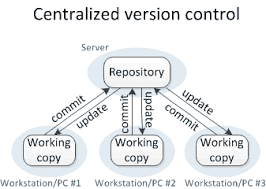
\includegraphics[width=10cm,height=7cm]{Figures/stash.jpg}}
	\caption{Version Control System}
	\label{stash.jpg}
\end{figure}

Version Control System (VCS) adalah perangkat lunak yang membantu 
pengembang perangkat lunak untuk bekerja sama dan menjaga sejarah 
lengkap dari pekerjaan mereka.

\begin{table}[ht]
	\caption{Fungsi VCS}
	\centering
	\begin{tabular}{cccc}
		\hline
		No&Keterangan&\\
		\hline
		.1&Memungkinkan pengembang untuk bekerja secara bersamaan&\\
		.2&Tidak memungkinkan Timpa perubahan masing-masing&\\
		.3&Mempertahankan sejarah setiap versi&\\
		\hline
	\end{tabular}
\end{table}


Berikut ini adalah jenis VCS:

\begin{itemize}
\item sistem kontrol versi terpusat (CVCS).
\item Didistribusikan / Desentralisasi sistem kontrol versi (DVCS).
\end{itemize}
Dalam bab ini, kita akan berkonsentrasi hanya pada sistem kontrol versi 
didistribusikan dan terutama pada Git. Git berada di bawah sistem 
kontrol versi terdistribusi.

\subsection{Distributed Sistem Kontrol Versi}
sistem terpusat kontrol versi (CVCS) menggunakan server pusat untuk 
menyimpan semua file dan memungkinkan kolaborasi tim. Tapi kelemahan 
utama dari CVCS adalah titik tunggal kegagalan, yaitu, kegagalan server 
pusat. Sayangnya, jika server pusat turun selama satu jam, kemudian pada 
jam itu, tidak ada yang bisa berkolaborasi sama sekali. Dan bahkan dalam 
kasus terburuk, jika disk server pusat akan rusak dan cadangan yang 
tepat belum diambil, maka Anda akan kehilangan seluruh sejarah proyek. 
Di sini, sistem terdistribusi kontrol versi (DVCS) datang ke dalam 
gambar.\vspace{14pt}

DVCS klien tidak hanya memeriksa snapshot terbaru dari direktori tetapi 
mereka juga penuh dari repositori tersebut. Jika memutuskan turun, maka 
repositori dari klien dapat disalin kembali ke server untuk 
mengembalikannya. Setiap checkout adalah salinan lengkap dari 
repositori. Git tidak bergantung pada server pusat dan itulah sebabnya 
Anda dapat melakukan banyak operasi ketika Anda sedang offline. Anda 
dapat melakukan perubahan, membuat cabang, lihat log, dan melakukan 
operasi lain ketika Anda sedang offline. Anda memerlukan koneksi 
jaringan hanya untuk mempublikasikan perubahan dan mengambil perubahan 
terbaru.

\subsection{Keuntungan dari Git}\vspace{14pt}

{\textbf{free dan open source}}\vspace{14pt}

Git dirilis di bawah lisensi open source GPL ini. Ini tersedia secara 
bebas melalui internet. Anda dapat menggunakan Git untuk mengelola 
proyek kepatutan tanpa membayar satu sen dolar. Karena merupakan open 
source, Anda dapat men-download kode sumbernya dan juga melakukan 
perubahan sesuai dengan kebutuhan Anda.\vspace{14pt}


{\textbf{Cepat dan kecil}}\vspace{14pt}

Karena sebagian besar operasi dilakukan secara lokal, memberikan manfaat 
yang sangat besar dalam hal kecepatan. Git tidak bergantung pada server 
pusat; itu sebabnya, tidak ada kebutuhan untuk berinteraksi dengan 
server remote untuk setiap operasi. Bagian inti dari Git ditulis dalam 
C, yang menghindari overhead runtime yang terkait dengan bahasa tingkat 
tinggi lainnya. Meskipun Git cermin seluruh repositori, ukuran data di 
sisi client kecil. Ini menggambarkan efisiensi Git di mengompresi dan 
menyimpan data di sisi client.\vspace{14pt}


	{\textbf{backup implisit}}\vspace{14pt}

Kemungkinan kehilangan data sangat jarang ketika ada beberapa salinan 
dari itu. Data hadir di setiap sisi klien cermin repositori, karena itu 
dapat digunakan dalam hal terjadi kecelakaan atau korupsi disk.\vspace{14pt}


{\textbf{Keamanan}}\vspace{14pt}

Git menggunakan fungsi hash kriptografi umum yang disebut fungsi hash 
aman (SHA1), untuk nama dan mengidentifikasi objek dalam database. 
Setiap file dan komit check-dijumlahkan dan diambil oleh checksum-nya 
pada saat checkout. Ini menyiratkan bahwa, tidak mungkin untuk mengubah 
file, tanggal, dan pesan komit dan data lainnya dari database Git tanpa 
mengetahui Git.\vspace{14pt}


	{\textbf{Tidak perlu perangkat keras yang kuat}}\vspace{14pt}

Dalam kasus CVCS, server pusat harus cukup kuat untuk melayani 
permintaan dari seluruh tim. Untuk tim yang lebih kecil, itu tidak 
masalah, tetapi sebagai ukuran tim tumbuh, keterbatasan hardware server 
dapat menjadi hambatan kinerja. Dalam kasus DVCS, pengembang tidak 
berinteraksi dengan server kecuali mereka butuhkan untuk mendorong atau 
menarik perubahan. Semua angkat berat terjadi pada sisi klien, sehingga 
hardware server dapat memang sangat sederhana.\vspace{14pt}


{\textbf{percabangan mudah}\vspace{14pt}

CVCS menggunakan mekanisme copy murah, Jika kita membuat cabang baru, 
itu akan menyalin semua kode ke cabang baru, sehingga memakan waktu dan 
tidak efisien. Juga, penghapusan dan penggabungan cabang di CVCS rumit 
dan memakan waktu. Tapi manajemen cabang dengan Git sangat sederhana. 
Dibutuhkan hanya beberapa detik untuk membuat, menghapus, dan 
menggabungkan cabang.






\chapter{Move Operation}
\section{Move Operation}
\hspace*{0.5in}Seperti namanya, operasi memindahkan direktori atau file dari satu lokasi ke lokasi lain. direktori yang dimodifikasi akan muncul sebagai berikut: \par
\vspace{10pt}
\begin{verbatim}
[tom@CentOS project] $  \$  $ pwd} 

/home/tom/project} 
[tom@CentOS project] $  \$  $ ls} 

{README string string.c} 
[tom@CentOS project] $  \$  $ mkdir src

[tom@CentOS project] $  \$  $ git mv string.c src/} 

[tom@CentOS project] $  \$  $ git status -s

R string.c  $ - $> src/string.c

?? string}
\end{verbatim}

\vspace{10pt}
\hspace*{0.5in} Untuk membuat perubahan ini permanen, harus mendorong struktur direktori yang dimodifikasi ke repositori jauh sehingga pengembang lain dapat melihat ini. \par

\noindent 
[tom@CentOS project] $  \$  $ git commit -m "Modified directory structure" \par
\vspace{12pt}
\noindent 
[master 7d9ea97] Modified directory structure \par
\noindent 
1 files changed, 0 insertions(+), 0 deletions(-) \par
\noindent 
rename string.c => src/string.c (100 $  \%  $) \par
\vspace{12pt}
\noindent 
[tom@CentOS project] $  \$  $ git push origin master \par
\noindent 
Counting objects: 4, done. \par
\noindent 
Compressing objects: 100 $  \%  $ (2/2), done. \par
\noindent 
Writing objects: 100 $  \%  $ (3/3), 320 bytes, done. \par
\noindent 
Total 3 (delta 0), reused 0 (delta 0) \par
\noindent 
To gituser@git.server.com:project.git \par
\noindent 
e86f062..7d9ea97 master  $ - $> master \par

\vspace{12pt}
\hspace*{0.5in} Di gudang lokal Jerry, sebelum operasi penarikan, ia akan menunjukkan struktur direktori lama. \par

\vspace{12pt}
\noindent 
[jerry@CentOS project] $  \$  $ pwd \par
\noindent 
/home/jerry/jerry $  \_  $repo/project \par
\vspace{12pt}
\noindent 
[jerry@CentOS project] $  \$  $ ls \par
\noindent 
README string string.c \par

\vspace{12pt}
\noindent 
 \hspace*{0.5in} Tapi setelah operasi tarik, struktur direktori akan diperbarui. Sekarang, Jerry bisa melihat direktori src dan file yang ada di dalam direktori itu. \par
\noindent 
[jerry@CentOS project] $  \$  $ git pull \par
\noindent 
remote: Counting objects: 4, done. \par
\noindent 
remote: Compressing objects: 100 $  \%  $ (2/2), done. \par
\noindent 
remote: Total 3 (delta 0), reused 0 (delta 0) \par
\noindent 
Unpacking objects: 100 $  \%  $ (3/3), done. \par
\noindent 
From git.server.com:project \par
\noindent 
e86f062..7d9ea97 master  $ - $> origin/master \par
\noindent 
First, rewinding head to replay your work on top of it... \par
\noindent 
Fast-forwarded master to 7d9ea97683da90bcdb87c28ec9b4f64160673c8a. \par
\vspace{12pt}
\noindent 
[jerry@CentOS project] $  \$  $ ls \par
\noindent 
README src string \par
\vspace{12pt}
\noindent 
[jerry@CentOS project] $  \$  $ ls src/ \par
\noindent 
string.c \par

\subsection{Semua Operasi Dilakukan Secara Lokal}
\par
\hspace*{0.5in} Kebanyakan operasi pada Git hanya membutuhkan berkas-berkas dan resource lokal – tidak ada informasi yang dibutuhkan dari komputer lain pada jaringan. Jika terbiasa dengan VCS terpusat dimana kebanyakan operasi memiliki overhead latensi jaringan, aspek Git satu ini akan membuat berpikir bahwa para dewa kecepatan telah memberkati Git dengan kekuatan. Karena memiliki seluruh sejarah dari proyek di lokal disk, dengan kebanyakan operasi yang tampak hampir seketika. \par
\hspace*{0.5in} Sebagai contoh, untuk melihat history dari proyek, Git tidak membutuhkan data histori dari server untuk kemudian menampilkannya untuk, namun secara sedarhana Git membaca historinya langsung dari basisdata lokal proyek tersebut. Ini berarti melihat histori proyek hampir secara instant. Jika ingin membandingkan perubahan pada sebuah berkas antara versi saat ini dengan versi sebulan yang lalu, Git dapat mencari berkas yang sama pada sebulan yang lalu dan melakukan pembandingan perubahan secara lokal, bukan dengan cara meminta remote server melakukannya atau meminta server mengirimkan berkas versi yang lebih lama kemudian membandingkannya secara lokal. \par
\hspace*{0.5in} Hal ini berarti bahwa sangat sedikit yang tidak bisa kerjakan jika sedang offline atau berada diluar VPN. Jika sedang berada dalam pesawat terbang atau sebuah kereta dan ingin melakukan pekerjaan kecil, dapat melakukan commit sampai memperoleh koneksi internet hingga dapat menguploadnya. Jika pulang ke rumah dan VPN client tidak bekerja dengan benar, tetap dapat bekerja. Pada kebanyakan sistem lainnya, melakukan hal ini cukup sulit atau bahkan tidak mungkin sama sekali. Pada Perforce misalnya, tidak dapat berbuat banyak ketika tidak terhubung dengan server; pada Subversion dan CVS,  dapat mengubah berkas, tapi tidak dapat melakukan commit pada basisdata (karena tidak terhubung dengan basisdata). Hal ini mungkin saja bukanlah masalah yang besar, namun akan terkejut dengan perbedaan besar yang disebabkannya. \par

\subsection{Git Memiliki Integritas }
\par
\hspace*{0.5in} Segala sesuatu pada Git akan melalui proses checksum terlebih dahulu sebelum disimpan yang kemudian direferensikan oleh hasil checksum tersebut. Hal ini berarti tidak mungkin melakukan perubahan terhadap berkas manapun tanpa diketahui oleh Git. Fungsionalitas ini dimiliki oleh Git pada level terendahnya dan ini merupakan bagian tak terpisahkan dari filosofi Git. Tidak akan kehilangan informasi atau mendapatkan file yang cacat tanpa diketahui oleh Git. \par
\hspace*{0.5in} Mekanisme checksum yang digunakan oleh Git adalah SHA-1 hash. Ini merupakan sebuah susunan string yang terdiri dari 40 karakter heksadesimal (0 hingga 9 dan a hingga f) dan dihitung berdasarkan isi dari sebuah berkas atau struktur direktori pada Git. sebuah hash SHA-1 berupa seperti berikut: \par
\noindent 
24b9da6552252987aa493b52f8696cd6d3b00373 \par
\vspace{12pt}
\hspace*{0.5in}Nilai seperti ini pada berbagai tempat di Git. Faktanya, Git tidak menyimpan nama berkas pada basisdatanya, melainkan nilai hash dari isi berkas. \par
\hspace*{0.5in} Ketika melakukan operasi pada Git, kebanyakan dari operasi tersebut hanya menambahkan data pada basisdata Git. Seperti pada berbagai VCS, dapat kehilangan atau mengacaukan perubahan yang belum di-commit; namun jika melakukan commit pada Git akan sangat sulit kehilangannya, terutama jika  secara teratur melakukan push basisdata pada repositori lain. \par
\hspace*{0.5in} Hal ini menjadikan Git menyenangkan karena kita dapat berexperimen tanpa kehawatiran untuk mengacaukan proyek. Git memiliki 3 keadaan utama dimana berkas dapat berada: committed, modified dan staged. Committed berarti data telah tersimpan secara aman pada basisdata lokal. Modified berarti telah melakukan perubahan pada berkas namun belum melakukan commit pada basisdata. Staged berarti telah menandai berkas yang telah diubah pada versi yang sedang berlangsung untuk kemudian dilakukan commit. \par
\hspace*{0.5in} Direktori Git adalah dimana Git menyimpan metadata dan database objek untuk projek. Ini adalah bahagian terpenting dari Git, dan inilah yang disalin ketika melakukan kloning sebuah repository dari komputer lain. \par
\noindent 
\hspace*{0.5in} Direktori kerja adalah sebuah checkout tunggal dari satu versi dari projek. Berkas-berkas ini kemudian ditarik keluar dari basisdata yang terkompresi dalam direktori Git dan disimpan pada disk untuk gunakan atau modifikasi. \par
\hspace*{0.5in} Staging area adalah sebuah berkas sederhana, umumnya berada dalam direktori Git, yang menyimpan informasi mengenai apa yang menjadi commit selanjutnya. Ini terkadang disebut sebagai index, tetapi semakin menjadi standard untuk menyebutnya sebagai staging area.Alur kerja dasar Git adalah seperti ini: \par
\noindent 
 \par
\hspace*{0.5in} Jika sebuah versi tertentu dari sebuah berkas telah ada di direktori git dianggap 'committed'. Jika berkas diubah (modified) tetapi sudah ditambahkan ke staging area  maka itu adalah 'staged'. Dan jika berkas telah diubah sejak terakhir dilakukan checked out tetapi belum ditambahkan ke staging area maka itu adalah 'modified'.  \par

\subsection*{13.3 Perintah Untuk Membuat Sebuah Proyek }
\hspace*{0.5in} Membuat direktori baru di repositori Git dengan git init. Melakukan direktori setiap saat, benar-benar lokal. Executive git init dalam direktori, Membuat Git repositori. Sebagai contoh, buat item w3big:  \par
\noindent 
{\fontsize{10pt}{10pt}\selectfont  $  \$  $ mkdir w3big} \par
\noindent 
{\fontsize{10pt}{10pt}\selectfont  $  \$  $ cd w3big/} \par
\noindent 
{\fontsize{10pt}{10pt}\selectfont  $  \$  $ git init} \par
\noindent 
{\fontsize{10pt}{10pt}\selectfont Initialized empty Git repository in /Users/tianqixin/www/w3big/.git/} \par
\noindent 
{\fontsize{10pt}{10pt}\selectfont  $  \#  $ 在 /www/w3big/.git/ 目录初始化空 Git 仓库完毕。} \par
\vspace{14pt}
\hspace*{0.5in} Sekarang dapat melihat subdirektori git yang dihasilkan dalam proyek. Ini adalah repositori Git, dan semua data yang terkait dengan snapshot dari proyek disimpan di sini. \par
\noindent 
{\fontsize{10pt}{10pt}\selectfont ls -a} \par

\vspace{12pt}
\hspace*{0.5in} Gunakan git clone repositori Git untuk salinan lokal, sehingga dapat melihat item atau memodifikasinya. Jika membutuhkan sebuah proyek kerjasama dengan orang lain atau ingin menyalin sebuah proyek, melihat kode, dapat mengkloning proyek. Jalankan:  \par
\noindent 
{\fontsize{10pt}{10pt}\selectfont git clone [url]} \par
\vspace{12pt}
\noindent 
Sebagai contoh, kloning proyek pada Github: \par
\noindent 
{\fontsize{10pt}{10pt}\selectfont  $  \$  $ git clone git@github.com:schacon/simplegit.git} \par
\noindent 
{\fontsize{10pt}{10pt}\selectfont Cloning into 'simplegit'...} \par
\noindent 
{\fontsize{10pt}{10pt}\selectfont remote: Counting objects: 13, done.} \par
\noindent 
{\fontsize{10pt}{10pt}\selectfont remote: Total 13 (delta 0), reused 0 (delta 0), pack-reused 13} \par
\noindent 
{\fontsize{10pt}{10pt}\selectfont Receiving objects: 100 $  \%  $ (13/13), done.} \par
\noindent 
{\fontsize{10pt}{10pt}\selectfont Resolving deltas: 100 $  \%  $ (2/2), done.} \par
\noindent 
{\fontsize{10pt}{10pt}\selectfont Checking connectivity... done.} \par
\vspace{12pt}
\noindent 
\hspace*{0.5in} Setelah kloning selesai di direktori saat ini akan menghasilkan simplegit direktori:  \par
\noindent 
{\fontsize{10pt}{10pt}\selectfont  $  \$  $ Cd simplegit /  $  \$  $ ls README Rakefile lib } \par
\noindent 
operasi akan menyalin semua catatan proyek.  \par
\vspace{12pt}
\noindent 
{\fontsize{10pt}{10pt}\selectfont  $  \$  $ ls -a} \par
\noindent 
{\fontsize{10pt}{10pt}\selectfont git~~~~ README   Rakefile lib} \par
\noindent 
{\fontsize{10pt}{10pt}\selectfont  $  \$  $ cd .git} \par
\noindent 
{\fontsize{10pt}{10pt}\selectfont  $  \$  $ ls} \par
\noindent 
{\fontsize{10pt}{10pt}\selectfont HEAD~~~~~~~~description~info~~~~~   packed-refs} \par
\noindent 
{\fontsize{10pt}{10pt}\selectfont branches~~~~hooks~~~~~~~logs~~~~~   refs} \par
\noindent 
{\fontsize{10pt}{10pt}\selectfont config~~~~~~index~~~~~  objects} \par
\vspace{12pt}
\hspace*{0.5in}Secara default, Git akan mengikuti nama URL yang tersedia item untuk membuat direktori proyek lokalditunjukkan. URL biasanya nama item terakhir / setelah. Jika ingin nama yang berbeda  dapat menambahkan nama yang inginkan setelah perintah. \par

\subsection*{13.4 Snapshot Dasar }
 \par
\hspace*{0.5in} Pekerjaan Git adalah untuk membuat dan menyimpan snapshot dari proyek dan setelah snapshot dan membandingkan. Bab ini akan tentang menciptakan sebuah snapshot dari proyek  dan mengirimkan pengenalan perintah. Git add perintah untuk menambahkan file ke cache, seperti yang tambahkan dua file berikut: \par
\noindent 
{\fontsize{10pt}{10pt}\selectfont  $  \$  $ touch README} \par
\noindent 
{\fontsize{10pt}{10pt}\selectfont  $  \$  $ touch hello.php} \par
\noindent 
{\fontsize{10pt}{10pt}\selectfont  $  \$  $ ls} \par
\noindent 
{\fontsize{10pt}{10pt}\selectfont README hello.php} \par
\noindent 
{\fontsize{10pt}{10pt}\selectfont  $  \$  $ git status -s} \par
\noindent 
{\fontsize{10pt}{10pt}\selectfont ?? README} \par
\noindent 
{\fontsize{10pt}{10pt}\selectfont ?? hello.php} \par
\noindent 
{\fontsize{10pt}{10pt}\selectfont  $  \$  $ } \par
\vspace{12pt}
\noindent 
 \hspace*{0.5in}Perintah git status digunakan untuk melihat status proyek. Selanjutnya jalankan git add perintah untuk menambahkan file: } \par
\noindent 
{\fontsize{10pt}{10pt}\selectfont  $  \$  $ git add README hello.php } \par

\vspace{12pt}
\hspace*{0.5in} Sekarang jalankan git status, dapat melihat dua dokumen tersebut telah ditambahkan untuk pergi : \par
\noindent 
{\fontsize{10pt}{10pt}\selectfont  $  \$  $ git status -s} \par
\noindent 
{\fontsize{10pt}{10pt}\selectfont A~ README} \par
\noindent 
{\fontsize{10pt}{10pt}\selectfont A~ hello.php} \par
\noindent 
{\fontsize{10pt}{10pt}\selectfont  $  \$  $ } \par

\vspace{12pt}
\hspace*{0.5in} Proyek baru, menambahkan semua file yang sama, kita dapat menggunakangit add. Perintah untuk menambahkan semua file dalam proyek saat ini. Sekarang memodifikasi file README:   \par
\noindent 
{\fontsize{10pt}{10pt}\selectfont  $  \$  $ vim README} \par
\noindent 
{\fontsize{10pt}{10pt}\selectfont <pre>} \par
\noindent 
{\fontsize{10pt}{10pt}\selectfont <p>在 README 添加以下内容:<b> $  \#  $ w3big Git 测试</b>,然后保存退出。</p>} \par
\noindent 
{\fontsize{10pt}{10pt}\selectfont <p>再执行一下 git status:</p>} \par
\noindent 
{\fontsize{10pt}{10pt}\selectfont  $  \$  $ git status -s} \par
\noindent 
{\fontsize{10pt}{10pt}\selectfont AM README} \par
\noindent 
{\fontsize{10pt}{10pt}\selectfont A~ hello.php} \par
\vspace{12pt}
\hspace*{0.5in}"AM" status berarti bahwa file tersebut setelah kami menambahkannya ke cache ada perubahan. Setelah perubahan menjalankan git add perintah untuk menambahkannya ke cache: \par
\noindent 
{\fontsize{10pt}{10pt}\selectfont  $  \$  $ git add .} \par
\noindent 
{\fontsize{10pt}{10pt}\selectfont  $  \$  $ git status -s} \par
\noindent 
{\fontsize{10pt}{10pt}\selectfont A~ README} \par
\noindent 
{\fontsize{10pt}{10pt}\selectfont A~ hello.php} \par
\vspace{12pt}
\hspace*{0.5in} Bila ingin perubahan yang terkandung dalam snapshot laporan yang akan datang dalam waktu, harus menjalankan git add. \par
\hspace*{0.5in} Git status untuk melihat setelah komit terakhir jika ada perubahan. Menunjukkan perintah ini ketika ditambahkan -s parameter untuk mendapatkan hasil yang singkat. Jika  tidak menambahkan parameter ini akan keluaran rinci:  \par
\noindent 
~  $  \$  $ git status \par
\noindent 
{\fontsize{10pt}{10pt}\selectfont On branch master} \par
\noindent 
\vspace{10pt}
\noindent 
{\fontsize{10pt}{10pt}\selectfont Initial commit} \par
\noindent 
\vspace{10pt}

\vspace{80pt}
{\fontsize{10pt}{10pt}\selectfont Changes to be committed:} \par
\noindent 
{\fontsize{10pt}{10pt}\selectfont ~ (use "git rm --cached <file>..." to unstage)} \par
\noindent 
\vspace{10pt}
\noindent 
{\fontsize{10pt}{10pt}\selectfont  \hspace*{0.64in} new~file:~  README} \par
\noindent 
{\fontsize{10pt}{10pt}\selectfont  \hspace*{0.64in} new~file:~  hello.php} \par
\vspace{12pt}
\hspace*{0.5in} Status git diff git eksekutif untuk melihat rincian hasil eksekusi. Git perintah diff dan menampilkan cache write telah dimodifikasi tapi belum ditulis ke cache perubahan perbedaan. git diff Ada dua skenario utama.  \par
\noindent 
\begin{itemize}
\item Perubahan tidak cache:diff git  \par
\noindent 
\item Lihatperubahan cache: git diff --cached \par
\noindent 
\item Lihat cache dan uncached semuaperubahan: git diff KEPALA \par
\noindent 
\item Tampilkan ringkasan daripada seluruhdiff: git diff --stat\end{itemize}
 \par
 

\vspace{12pt}
\noindent 
Masukkan berikut dalam file hello.php:  \par
\begin{verbatim}
<?php
echo 'www.w3big.com';
?>
git status -s
A README
AM hello.php
git diff
diff --git a/hello.php b/hello.php
index e69de29..69b5711 100644
--- a/hello.php
+++ b/hello.php
@@ -0,0 +1,3 @@
+<?php
+echo ':www.w3big.com';
+?>
\end{verbatim}

\vspace{10pt}
\hspace*{0.5in}Menampilkan status git pada untuk berubah setelah update atau menulis garis perubahan cache dengan garis dan git diff menunjukkan secara spesifik apa perubahan tersebut.  Selanjutnya melihat git berikutnya diff pelaksanaan --cached hasil:  \par
\noindent 
{\fontsize{10pt}{10pt}\selectfont  $  \$  $ git add hello.php } \par
\noindent 
{\fontsize{10pt}{10pt}\selectfont  $  \$  $ git status -s} \par
\noindent 
{\fontsize{10pt}{10pt}\selectfont A~ README} \par
\noindent 
{\fontsize{10pt}{10pt}\selectfont A~ hello.php} \par
\noindent 
{\fontsize{10pt}{10pt}\selectfont  $  \$  $ git diff --cached} \par
\noindent 
{\fontsize{10pt}{10pt}\selectfont diff --git a/README b/README} \par
\noindent 
{\fontsize{10pt}{10pt}\selectfont new file mode 100644} \par
\noindent 
{\fontsize{10pt}{10pt}\selectfont index 0000000..8f87495} \par
\noindent 
{\fontsize{10pt}{10pt}\selectfont --- /dev/null} \par
\noindent 
{\fontsize{10pt}{10pt}\selectfont +++ b/README} \par
\noindent 
{\fontsize{10pt}{10pt}\selectfont @@ -0,0 +1 @@} \par
\noindent 
{\fontsize{10pt}{10pt}\selectfont + $  \#  $ w3big Git 测试} \par
\noindent 
{\fontsize{10pt}{10pt}\selectfont diff --git a/hello.php b/hello.php} \par
\noindent 
{\fontsize{10pt}{10pt}\selectfont new file mode 100644} \par
\noindent 
{\fontsize{10pt}{10pt}\selectfont index 0000000..69b5711} \par
\noindent 
{\fontsize{10pt}{10pt}\selectfont --- /dev/null} \par
\noindent 
{\fontsize{10pt}{10pt}\selectfont +++ b/hello.php} \par
\noindent 
{\fontsize{10pt}{10pt}\selectfont @@ -0,0 +1,3 @@} \par
\noindent 
{\fontsize{10pt}{10pt}\selectfont +<?php} \par
\noindent 
{\fontsize{10pt}{10pt}\selectfont +echo '本教程:www.w3big.com';} \par
\noindent 
{\fontsize{10pt}{10pt}\selectfont +?>} \par
\vspace{12pt}
\hspace*{0.5in} Gunakan git menambahkan perintah ingin menulis isi dari buffer snapshot, dan mengeksekusi git commit akan menambahkan konten ke gudang penyangga. Git mengirimkan masing-masing nama dan alamat e-mail yang tercatat, sehingga langkah pertama perlu mengkonfigurasi nama pengguna dan alamat e-mail.  \par
\noindent 
{\fontsize{10pt}{10pt}\selectfont  $  \$  $ git config --global user.name 'w3big'} \par
\noindent 
{\fontsize{10pt}{10pt}\selectfont  $  \$  $ git config --global user.email test@w3big.com} \par
\vspace{12pt}
\hspace*{0.5in} Berikutnya menulis caching, dan menyerahkan semua perubahan hello.php tersebut. Dalam contoh pertama menggunakan opsi -m untuk memberikan baris perintah untuk mengirimkan komentar : \par
\noindent 
{\fontsize{10pt}{10pt}\selectfont  $  \$  $ git add hello.php} \par
\noindent 
{\fontsize{10pt}{10pt}\selectfont  $  \$  $ git status -s} \par
\noindent 
{\fontsize{10pt}{10pt}\selectfont A~ README} \par
\noindent 
{\fontsize{10pt}{10pt}\selectfont A~ hello.php} \par
\noindent 
{\fontsize{10pt}{10pt}\selectfont  $  \$  $  $  \$  $ git commit -m '第一次版本提交'} \par
\noindent 
{\fontsize{10pt}{10pt}\selectfont [master (root-commit) d32cf1f] 第一次版本提交} \par
\noindent 
{\fontsize{10pt}{10pt}\selectfont  2 files changed, 4 insertions(+)} \par
\noindent 
{\fontsize{10pt}{10pt}\selectfont  create mode 100644 README} \par
\noindent 
{\fontsize{10pt}{10pt}\selectfont  create mode 100644 hello.php} \par
\noindent 
{\fontsize{10pt}{10pt}\selectfont  } \par

\vspace{12pt}
Sekarang telah mencatat snapshot. Jika di jalankan git status:  \par
\noindent 
{\fontsize{10pt}{10pt}\selectfont  $  \$  $ git status} \par
\noindent 
{\fontsize{10pt}{10pt}\selectfont  $  \#  $ On branch master} \par
\noindent 
{\fontsize{10pt}{10pt}\selectfont nothing to commit (working directory clean)} \par
\vspace{12pt}
\hspace*{0.5in} Output di atas menunjukkan bahwa setelah pengajuan terakhir, tidak membuat perubahan apapu. Jika tidak menetapkan opsi -m, Git mencoba untuk membuka editor untuk mengisi informasi yang disampaikan. Git jika tidak dapat menemukan informasi yang relevan dalam konfigurasi, default akan membuka vim. Layar akan terlihat seperti ini:  \par
\noindent 
{\fontsize{10pt}{10pt}\selectfont  $  \#  $ Please enter the commit message for your changes. Lines starting} \par
\noindent 
{\fontsize{10pt}{10pt}\selectfont  $  \#  $ with ' $  \#  $' will be ignored, and an empty message aborts the commit.} \par
\noindent 
{\fontsize{10pt}{10pt}\selectfont  $  \#  $ On branch master} \par
\noindent 
{\fontsize{10pt}{10pt}\selectfont  $  \#  $ Changes to be committed:} \par
\noindent 
{\fontsize{10pt}{10pt}\selectfont  $  \#  $~~ (use "git reset HEAD <file>..." to unstage)} \par
\noindent 
{\fontsize{10pt}{10pt}\selectfont  $  \#  $} \par
\noindent 
{\fontsize{10pt}{10pt}\selectfont  $  \#  $~modified:~  hello.php} \par
\noindent 
{\fontsize{10pt}{10pt}\selectfont  $  \#  $} \par
\noindent 
{\fontsize{10pt}{10pt}\selectfont  $  \sim  $} \par
\noindent 
{\fontsize{10pt}{10pt}\selectfont  $  \sim  $} \par
\noindent 
{\fontsize{10pt}{10pt}\selectfont ".git/COMMIT $  \_  $EDITMSG" 9L, 257C} \par
\vspace{12pt}
\hspace*{0.5in} Jika berpikir git add disampaikan proses cache yang terlalu rumit, Git juga memungkinkan untuk menggunakan opsi -a untuk melewatkan langkah ini. format perintah adalah sebagai berikut: \par
\noindent 
{\fontsize{10pt}{10pt}\selectfont git commit -a} \par
\vspace{12pt}
\noindent 
Memodifikasi file hello.php sebagai berikut:  \par
\noindent 
{\fontsize{10pt}{10pt}\selectfont <?php} \par
\noindent 
{\fontsize{10pt}{10pt}\selectfont echo '本教程:www.w3big.com';} \par
\noindent 
{\fontsize{10pt}{10pt}\selectfont echo '本教程:www.w3big.com';} \par
\noindent 
{\fontsize{10pt}{10pt}\selectfont ?>} \par
\vspace{10pt}
\noindent 
Kemudian jalankan perintah berikut:  \par
\noindent 
{\fontsize{10pt}{10pt}\selectfont git commit -am '修改 hello.php 文件'} \par
\noindent 
{\fontsize{10pt}{10pt}\selectfont [master 71ee2cb] 修改 hello.php 文件} \par
\noindent 
{\fontsize{10pt}{10pt}\selectfont  1 file changed, 1 insertion(+)} \par
\vspace{10pt}
\hspace*{0.5in} Git reset perintah HEAD untuk menghapus konten cache.  Mari mengubah file berkas README, sebagai berikut:  \par
\noindent 
{\fontsize{10pt}{10pt}\selectfont  $  \#  $ w3big Git 测试} \par
\noindent 
{\fontsize{10pt}{10pt}\selectfont  $  \#  $ 本教程 } \par
\vspace{12pt}
\noindent 
File hello.php diubah sebagai berikut:  \par
\noindent 
{\fontsize{10pt}{10pt}\selectfont <?php} \par
\noindent 
{\fontsize{10pt}{10pt}\selectfont echo '本教程:www.w3big.com';} \par
\noindent 
{\fontsize{10pt}{10pt}\selectfont echo '本教程:www.w3big.com';} \par
\noindent 
{\fontsize{10pt}{10pt}\selectfont echo '本教程:www.w3big.com';} \par
\noindent 
{\fontsize{10pt}{10pt}\selectfont ?>} \par
\vspace{10pt}
\hspace*{0.5in} Sekarang setelah dua file diubah disampaikan ke zona penyangga, sekarang ingin membatalkan salah satu dari cache, sebagai berikut: \par
\noindent 
{\fontsize{10pt}{10pt}\selectfont  $  \$  $ git status -s} \par
\noindent 
{\fontsize{10pt}{10pt}\selectfont  M README} \par
\noindent 
{\fontsize{10pt}{10pt}\selectfont  M hello.php} \par
\noindent 
{\fontsize{10pt}{10pt}\selectfont  $  \$  $ git add .} \par
\noindent 
{\fontsize{10pt}{10pt}\selectfont  $  \$  $ git status -s} \par
\noindent 
{\fontsize{10pt}{10pt}\selectfont M~ README} \par
\noindent 
{\fontsize{10pt}{10pt}\selectfont M~ hello.pp} \par
\noindent 
{\fontsize{10pt}{10pt}\selectfont  $  \$  $ git reset HEAD -- hello.php } \par
\noindent 
{\fontsize{10pt}{10pt}\selectfont Unstaged changes after reset:} \par
\noindent 
{\fontsize{10pt}{10pt}\selectfont M \hspace*{0.64in} hello.php} \par
\noindent 
{\fontsize{10pt}{10pt}\selectfont  $  \$  $ git status -s} \par
\noindent 
{\fontsize{10pt}{10pt}\selectfont M~ README} \par
\noindent 
{\fontsize{10pt}{10pt}\selectfont  M hello.php} \par
\vspace{12pt}
\hspace*{0.5in} Sekarang menjalankan git commit, perubahan hanya akan diserahkan berkas README, tapi hello.php tidak.  \par
\noindent 
{\fontsize{10pt}{10pt}\selectfont  $  \$  $ git commit -m '修改'} \par
\noindent 
{\fontsize{10pt}{10pt}\selectfont [master f50cfda] 修改} \par
\noindent 
{\fontsize{10pt}{10pt}\selectfont  1 file changed, 1 insertion(+)} \par
\noindent 
{\fontsize{10pt}{10pt}\selectfont  $  \$  $ git status -s} \par
\noindent 
{\fontsize{10pt}{10pt}\selectfont  M hello.php} \par
\vspace{12pt}
\hspace*{0.5in} Melihat file perubahan hello.php dan untuk pengajuan. Maka dapat menggunakan perintah berikut untuk memodifikasi hello.php menyerahkan:  \par
\noindent 
{\fontsize{10pt}{10pt}\selectfont  $  \$  $ git commit -am '修改 hello.php 文件'} \par
\noindent 
{\fontsize{10pt}{10pt}\selectfont [master 760f74d] 修改 hello.php 文件} \par
\noindent 
{\fontsize{10pt}{10pt}\selectfont  1 file changed, 1 insertion(+)} \par
\noindent 
{\fontsize{10pt}{10pt}\selectfont  $  \$  $ git status} \par
\noindent 
{\fontsize{10pt}{10pt}\selectfont On branch master} \par
\noindent 
{\fontsize{10pt}{10pt}\selectfont nothing to commit, working directory clean} \par
\vspace{10pt}
\hspace*{0.5in} Singkatnya, melakukan git reset HEAD untuk membatalkan sebelum git add untuk menambahkan, tetapi tidak ingin untuk memasukkan dalam cache snapshot di commit selanjutnya. \par
\hspace*{0.5in} Entri rm git akan dihapus dari cache. ulang kepala git ini membatalkan entri cache yang berbeda. "Batal Cache", yang berarti bahwa pemulihan akan membuat perubahan ke cache.  Secara default, git file rm akan dihapus dari file cache dan hard drive  (direktori kerja). Jika ingin menyimpan file dalam direktori kerja, dapat menggunakangit rm --cached: Seperti kita menghapus hello.php file:  \par
\noindent 
{\fontsize{10pt}{10pt}\selectfont  $  \$  $ git rm hello.php } \par
\noindent 
{\fontsize{10pt}{10pt}\selectfont rm 'hello.php'} \par
\noindent 
{\fontsize{10pt}{10pt}\selectfont  $  \$  $ ls} \par
\noindent 
{\fontsize{10pt}{10pt}\selectfont README} \par

\vspace{50pt}
Tidak menghapus file dari ruang kerja:  \par
\noindent 
{\fontsize{10pt}{10pt}\selectfont  $  \$  $ git rm --cached README } \par
\noindent 
{\fontsize{10pt}{10pt}\selectfont rm 'README'} \par
\noindent 
{\fontsize{10pt}{10pt}\selectfont  $  \$  $ ls} \par
\noindent
{\fontsize{10pt}{10pt}\selectfont README} \par

\vspace{10pt}
\hspace*{0.5in} Git perintah mv untuk melakukan semua hal yanggit rm perintah operasi --cached,mengubah nama file pada disk, dan kemudian jalankan git add untuk menambahkan file baru ke cache.  README pertama kita hapus hanya menambahkan kembali:  \par
\noindent 
{\fontsize{10pt}{10pt}\selectfont  $  \$  $ git add README } \par
\vspace{12pt}
\noindent 
Kemudian nama yang sama yaitu:  \par
\noindent 
{\fontsize{10pt}{10pt}\selectfont  $  \$  $~git mv README  README.md} \par
\noindent 
{\fontsize{10pt}{10pt}\selectfont  $  \$  $ ls} \par
\noindent 
{\fontsize{10pt}{10pt}\selectfont README.md} 

\section{Mendapatkan File untuk Pindah}
\hspace*{0.5in} Buat salinan repositori A sehingga bisa memindahkannya tanpa terlalu mengkhawatirkan kesalahan. Sebaiknya hapus tautan ke repositori asli agar tidak sengaja membuat perubahan jarak jauh (baris 3). Ini berjalan melalui file, menghapus apapun yang tidak ada dalam direktori 1. Hasilnya adalah isi direktori 1 dipindahkan ke basis repositori A. Mengimpor file-file ini ke dalam repositori B di dalam direktori, jadi memindahkan semua menjadi satu sekarang (baris 5/6). Komit perubahan dan menggabungkan file-file ini ke dalam repositori yang baru \ref{PerpindahanFile} :
\begin{figure}[ht]
	\centerline{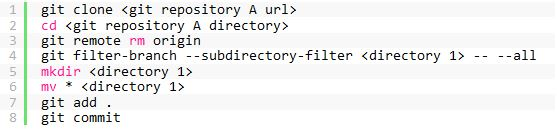
\includegraphics[width=0.50\textwidth]{Figures/PerpindahanFile}}
	\caption{PerpindahanFile}
	\label{PerpindahanFile}
\end{figure}

\chapter{Rename Operation}
Sampai sekarang, baik Tom dan Jerry menggunakan perintah manual untuk menyusun proyek mereka. Sekarang, Jerry memutuskan untuk membuat Makefile untuk proyek mereka dan juga memberi nama yang tepat untuk file "string.c". \par
\noindent 
{\fontsize{10pt}{10pt}\selectfont [jerry@CentOS project] $  \$  $ pwd} \par
\noindent 
{\fontsize{10pt}{10pt}\selectfont /home/jerry/jerry $  \_  $repo/project} \par
\noindent 
\vspace{10pt}
\noindent 
{\fontsize{10pt}{10pt}\selectfont [jerry@CentOS project] $  \$  $ ls} \par
\noindent 
{\fontsize{10pt}{10pt}\selectfont README src} \par
\noindent 
\vspace{10pt}
\noindent 
{\fontsize{10pt}{10pt}\selectfont [jerry@CentOS project] $  \$  $ cd src/} \par
\noindent 
\vspace{10pt}
\noindent 
{\fontsize{10pt}{10pt}\selectfont [jerry@CentOS src] $  \$  $ git add Makefile} \par
\noindent 
\vspace{10pt}
\noindent 
{\fontsize{10pt}{10pt}\selectfont [jerry@CentOS src] $  \$  $ git mv string.c string $  \_  $operations.c} \par
\noindent 
\vspace{10pt}
\noindent 
{\fontsize{10pt}{10pt}\selectfont [jerry@CentOS src] $  \$  $ git status -s} \par
\noindent 
{\fontsize{10pt}{10pt}\selectfont A Makefile} \par
\noindent 
{\fontsize{10pt}{10pt}\selectfont R string.c  $ - $> string $  \_  $operations.c} \par
\vspace{12pt}
Git menunjukkan R sebelum nama file untuk menunjukkan bahwa file telah diganti namanya. \par
Untuk komit operasi, Jerry menggunakan - bendera, yang membuat git komit secara otomatis mendeteksi file yang dimodifikasi. \par
\noindent 
[jerry@CentOS src] $  \$  $ git commit -a -m 'Added Makefile and renamed strings.c to \par
\noindent 
string $  \_  $operations.c ' \par
\vspace{12pt}
\noindent 
[master 94f7b26] Added Makefile and renamed strings.c to string $  \_  $operations.c \par
\noindent 
1 files changed, 0 insertions(+), 0 deletions(-) \par
\noindent 
create mode 100644 src/Makefile \par
\noindent 
rename src/ $  \{  $string.c => string $  \_  $operations.c $  \}  $ (100 $  \%  $) \par
\vspace{12pt}
\noindent 
Setelah komit, dia mendorong perubahannya ke repositori. \par
\noindent 
[jerry@CentOS src] $  \$  $ git push origin master \par
\vspace{12pt}
\noindent 
Perintah di atas akan menghasilkan hasil sebagai berikut: \par
\noindent 
Counting objects: 6, done. \par
\noindent 
Compressing objects: 100 $  \%  $ (3/3), done. \par
\noindent 
Writing objects: 100 $  \%  $ (4/4), 396 bytes, done. \par
\noindent 
Total 4 (delta 0), reused 0 (delta 0) \par
\noindent 
To gituser@git.server.com:project.git \par
\noindent 
7d9ea97..94f7b26 master  $ - $> master \par
\vspace{12pt}
Sekarang, pengembang lain dapat melihat modifikasi ini dengan memperbarui repositori lokal mereka. \par
Kegunaan utama dari sistem kontrol versi ialah sebagai alat untuk manajemen kode program. Terdapat dua kegunaan utama dari sistem ini, yaitu: \par
\noindent 
Menggabungkan perubahan-perubahan kode dari versi lama (misal: untuk mengembalikan fitur yang telah dihapus) ataupun menggabungkan perubahan dari orang lain (misal: menggabungkan fitur yang dikembangkan oleh anggota tim lain).
 \par
\vspace{12pt}
\noindent 
\textbf{14.1 Intalasi Git} \par
git berjalan pada semua sistem operasi populer (Mac, Windows, Linux). Jika menggunakan Windows atau Mac, masuk ke situs utama git pada 
 lalu lakukan download dan instalasi software tersebut. Pengguna Linux dapat melakukan instalasi melalui repositori distribusi yang dilakukan, melalui perintah sejenis: \par
\noindent 
{\fontsize{10pt}{10pt}\selectfont yum install git} \par
\vspace{12pt}
\noindent 
pada repositori berbasis RPM, atau perintah \par
\noindent 
{\fontsize{10pt}{10pt}\selectfont apt-get install git} \par
\vspace{12pt}
Untuk repositori berbasis deb. Kembali lagi, perintah hanya diberikan untuk distribusi paling populer (Debian / Ubuntu dan RedHat / Fedora), karena keterbatasan ruang. Jika menggunakan distrusi lain (seperti Gentoo atau Arch, maka diasumsikan telah mengetahui cara instalasi git atau perangkat lunak lain pada umumnya). \par
Khusus untuk sistem operasi Windows, pastikan instalasi anda diambil dari 
, karena pada paket yang tersedia di website tersebut telah diikutkan juga OpenSSH, yang akan sangat berguna jika ingin berkolaborasi dengan programmer lain. Perintah git juga harus memberikan respon yang benar: \par
\noindent 
{\fontsize{10pt}{10pt}\selectfont bert@LYNNSLENIA  $  \sim  $} \par
\noindent 
{\fontsize{10pt}{10pt}\selectfont  $  \$  $ git} \par
\noindent 
{\fontsize{10pt}{10pt}\selectfont usage: git [--version] [--exec-path[=<path>]] [--html-path] [--man-path] [--info-path]} \par
\noindent 
{\fontsize{10pt}{10pt}\selectfont ~~~~~~~~~~ [-p $  \vert  $--paginate $  \vert  $--no-pager] [--no-replace-objects] [--bare]} \par
\noindent 
{\fontsize{10pt}{10pt}\selectfont ~~~~~~~~~~ [--git-dir=<path>] [--work-tree=<path>] [--namespace=<name>]} \par
\noindent 
{\fontsize{10pt}{10pt}\selectfont ~~~~~~~~~~ [-c name=value] [--help]} \par
\noindent 
{\fontsize{10pt}{10pt}\selectfont ~~~~~~~~~~ <command> [<args>]} \par
\noindent 
{\fontsize{10pt}{10pt}\selectfont The most commonly used git commands are:} \par
\noindent 
{\fontsize{10pt}{10pt}\selectfont ~~~add~~~~~~  Add file contents to the index} \par
\noindent 
{\fontsize{10pt}{10pt}\selectfont ~~~bisect~~~  Find by binary search the change that introduced a bug} \par
\noindent 
{\fontsize{10pt}{10pt}\selectfont ~~~branch~~~  List, create, or delete branches} \par
\noindent 
{\fontsize{10pt}{10pt}\selectfont ~~~checkout~  Checkout a branch or paths to the working tree} \par
\noindent 
{\fontsize{10pt}{10pt}\selectfont ~~~clone~~~~  Clone a repository into a new directory} \par
\noindent 
{\fontsize{10pt}{10pt}\selectfont ~~~commit~~~  Record changes to the repository} \par
\noindent 
{\fontsize{10pt}{10pt}\selectfont ~diff~~~~~  Show changes between commits, commit and working tree, etc} \par
\noindent 
{\fontsize{10pt}{10pt}\selectfont ~~~fetch~~~~  Download objects and refs from another repository} \par
\noindent 
{\fontsize{10pt}{10pt}\selectfont ~~~grep~~~~~  Print lines matching a pattern} \par
\noindent 
{\fontsize{10pt}{10pt}\selectfont ~~~init~~~~~  Create an empty git repository or reinitialize an existing one} \par
\noindent 
{\fontsize{10pt}{10pt}\selectfont ~~~log~~~~~~  Show commit logs} \par
\noindent 
{\fontsize{10pt}{10pt}\selectfont ~~~merge~~~~  Join two or more development histories together} \par
\noindent 
{\fontsize{10pt}{10pt}\selectfont ~~~mv~~~~~~~  Move or rename a file, a directory, or a symlink} \par
\noindent 
{\fontsize{10pt}{10pt}\selectfont ~~~pull~~~~~  Fetch from and merge with another repository or a local branch} \par
\noindent 
{\fontsize{10pt}{10pt}\selectfont ~~~push~~~~~  Update remote refs along with associated objects} \par
\noindent 
{\fontsize{10pt}{10pt}\selectfont ~~~rebase~~~  Forward-port local commits to the updated upstream head} \par
\noindent 
{\fontsize{10pt}{10pt}\selectfont ~~~reset~~~~  Reset current HEAD to the specified state} \par
\noindent 
{\fontsize{10pt}{10pt}\selectfont ~~~rm~~~~~~~  Remove files from the working tree and from the index} \par
\noindent 
{\fontsize{10pt}{10pt}\selectfont ~~~show~~~~~  Show various types of objects} \par
\noindent 
{\fontsize{10pt}{10pt}\selectfont ~~~status~~~  Show the working tree status} \par
\noindent 
{\fontsize{10pt}{10pt}\selectfont ~~~tag~~~~~~  Create, list, delete or verify a tag object signed with GPG} \par
\noindent 
\vspace{10pt}
\noindent 
{\fontsize{10pt}{10pt}\selectfont See 'git help <command>' for more information on a specific command.} \par
\noindent 
{\fontsize{10pt}{10pt}\selectfont bert@LYNNSLENIA  $  \sim  $} \par
\noindent 
{\fontsize{10pt}{10pt}\selectfont  $  \$  $} \par
\vspace{12pt}
\noindent 
\textbf{14.2 Inisiasi} \par
Untuk dapat menggunakan sistem kontrol versi, terlebih dahulu kita harus mempersiapkan repositori. Sebuah repositori menyimpan seluruh versi dari kode program kita. Tidak usah takut, karena repositori tidak akan memakan banyak ruang \emph{hard disk}, karena penyimpanan tidak dilakukan terhadap keseluruhan file. Repositori hanya akan menyimpan \emph{perubahan} yang terjadi pada kode kita dari satu versi ke versi lainnya. Bahasa kerennya, repositori hanya menyimpan delta dari kode pada setiap versinya. \par
Pada (di saat kontrol versi yang populer adalah cvs dan programmer pada umumnya berjanggut putih), membangun repositori kode baru adalah hal yang sangat sulit dilakukan. Harus memiliki sebuah \emph{server} khusus yang dapat diakses oleh seluruh anggota tim. Jika server tidak dapat diakses karena jaringan rusak atau internet putus, maka tidak dapat melakukan kontrol versi (dan harus kembali ke metode direktori, atau tidak bekerja). \par
git merupakan sistem kontrol versi terdistribusi, yang berarti git dapat dijalankan tanpa perlu adanya repositori terpusat. Yang diperlukan untuk membuat repositori ialah mengetikkan perintah tertentu di direktori utama. Mulai membuat repositori baru.: \par
\noindent 
{\fontsize{10pt}{10pt}\selectfont bert@LYNNSLENIA  $  \sim  $} \par
\noindent 
{\fontsize{10pt}{10pt}\selectfont  $  \$  $ cd Desktop/projects/git-tutor/} \par
\noindent 
{\fontsize{10pt}{10pt}\selectfont bert@LYNNSLENIA  $  \sim  $/Desktop/projects/git-tutor} \par
\noindent 
{\fontsize{10pt}{10pt}\selectfont  $  \$  $ ls} \par
\noindent 
{\fontsize{10pt}{10pt}\selectfont bert@LYNNSLENIA  $  \sim  $/Desktop/projects/git-tutor} \par
\noindent 
{\fontsize{10pt}{10pt}\selectfont  $  \$  $} \par
\noindent 
\vspace{10pt}
Menambahkan kode baru ke dalam direktori ini. Buat sebuah file baru yang bernama cerita.txt di dalam direktori tersebut: \par
\noindent 
{\fontsize{10pt}{10pt}\selectfont bert@LYNNSLENIA  $  \sim  $/Desktop/projects/git-tutor} \par
\noindent 
{\fontsize{10pt}{10pt}\selectfont  $  \$  $ echo "ini adalah sebuah cerita" > cerita.txt} \par
\noindent 
\vspace{10pt}
\noindent 
{\fontsize{10pt}{10pt}\selectfont bert@LYNNSLENIA  $  \sim  $/Desktop/projects/git-tutor} \par
\noindent 
{\fontsize{10pt}{10pt}\selectfont  $  \$  $ ls} \par
\noindent 
{\fontsize{10pt}{10pt}\selectfont cerita.txt} \par
\vspace{12pt}
\noindent 
kemudian masukkan perintah git init untuk melakukan inisialisasi repositori: \par
\noindent 
{\fontsize{10pt}{10pt}\selectfont bert@LYNNSLENIA  $  \sim  $/Desktop/projects/git-tutor} \par
\noindent 
{\fontsize{10pt}{10pt}\selectfont  $  \$  $ git init} \par
\noindent 
{\fontsize{10pt}{10pt}\selectfont Initialized empty Git repository in c:/Users/bert/Desktop/projects/git-tutor/.git/} \par
\vspace{12pt}
Setelah melakukan inisialisasi, git secara otomatis akan membuat direktori .git pada repositori  (lihat potongan kode di bawah). Direktori tersebut merupakan direktori yang digunakan oleh git untuk menyimpan basis data delta kode, dan berbagai metadata lainnya. Mengubah direktori tersebut dapat menyebabkan hilangnya seluruh \emph{history} dari kode. \par
\noindent 
{\fontsize{10pt}{10pt}\selectfont bert@LYNNSLENIA  $  \sim  $/Desktop/projects/git-tutor (master)} \par
\noindent 
{\fontsize{10pt}{10pt}\selectfont  $  \$  $ ls -a} \par
\noindent 
{\fontsize{10pt}{10pt}\selectfont .~~..~ .git  cerita.txt} \par
\noindent 
\vspace{10pt}
\noindent 
\textbf{14.3 }\textbf{Penambahan File ke Repository} \par
\noindent 
 \hspace*{0.64in} Penyimpanan sejarah dapat dimulai dari saat pertama: kapan file tersebut dibuat dan ditambahkan ke dalam repositori. Untuk menambahkan file ke dalam repositori, gunakan perintah git add: \par
{\fontsize{10pt}{10pt}\selectfont bert@LYNNSLENIA  $  \sim  $/Desktop/projects/git-tutor (master)} \par
{\fontsize{10pt}{10pt}\selectfont  $  \$  $ git add .} \par
{\fontsize{10pt}{10pt}\selectfont warning: LF will be replaced by CRLF in cerita.txt.} \par
{\fontsize{10pt}{10pt}\selectfont The file will have its original line endings in your working directory.} \par
\noindent 
\vspace{12pt}
\noindent 
Secara sederhana, sintaks dari perintah git add adalah sebagai berikut: \par
{\fontsize{10pt}{10pt}\selectfont git add [nama file atau pola]} \par
\noindent 
\vspace{12pt}
\noindent 
 \hspace*{0.64in} Memasukkan nama file dalam perintah git add pada dasarnya akan memerintahkan git untuk menambahkan \textbf{semua} file baru dalam repositori. Jika hanya ingin menambahkan satu file (misalkan ada file yang belum yakin akan ditambahkan ke repositori), nama file spesifik dapat dimasukkan: \par
{\fontsize{10pt}{10pt}\selectfont git add cerita.txt} \par
\noindent 
\vspace{12pt}
Setelah menambahkan file ke dalam repositori, harus melakukan \emph{commit}. Perintah \emph{commit} memberitahukan kepada git untuk menyimpan sejarah dari file yang telah ditambahkan. Pada git, penambahan, perubahan, ataupun penghapusan sebuah file baru akan tercatat jika perntah \emph{commit} telah dijalankan. Mari lakukan \emph{commit} dengan menjalankan perintah git commit: \par
{\fontsize{10pt}{10pt}\selectfont bert@LYNNSLENIA  $  \sim  $/Desktop/projects/git-tutor (master)} \par
{\fontsize{10pt}{10pt}\selectfont  $  \$  $ git commit} \par
\noindent 
\vspace{12pt}
\noindent 
 \hspace*{0.64in} Jika langkah di atas diikuti dengan benar, maka kembali ke {\fontsize{11pt}{11pt}\selectfont git bash, dengan pesan berikut:} \par
{\fontsize{10pt}{10pt}\selectfont bert@LYNNSLENIA  $  \sim  $/Desktop/projects/git-tutor (master)} \par
{\fontsize{10pt}{10pt}\selectfont  $  \$  $ git commit} \par
{\fontsize{10pt}{10pt}\selectfont [master (root-commit) 1d4cdc9] Inisialisasi repo. Penambahan cerita.txt.} \par
{\fontsize{10pt}{10pt}\selectfont warning: LF will be replaced by CRLF in cerita.txt.} \par
{\fontsize{10pt}{10pt}\selectfont The file will have its original line endings in your working directory.} \par
{\fontsize{10pt}{10pt}\selectfont  1 file changed, 1 insertion(+)} \par
{\fontsize{10pt}{10pt}\selectfont  create mode 100644 cerita.txt} \par
\noindent 
\vspace{12pt}
\noindent 
\textbf{14.4}\textbf{ Mengubah Isi File} \par
Kegunaan utama kontrol versi (yang tercermin dari namanya) ialah melakukan manajemen perubahan secara otomatis untuk kita. dan kemudian jalankan perintah git commit lagi: \par
{\fontsize{10pt}{10pt}\selectfont bert@LYNNSLENIA  $  \sim  $/Desktop/projects/git-tutor (master)} \par
{\fontsize{10pt}{10pt}\selectfont  $  \$  $ git commit} \par
{\fontsize{10pt}{10pt}\selectfont  $  \#  $ On branch master} \par
{\fontsize{10pt}{10pt}\selectfont  $  \#  $ Changes not staged for commit:} \par
{\fontsize{10pt}{10pt}\selectfont  $  \#  $~~ (use "git add <file>..." to update what will be committed)} \par
{\fontsize{10pt}{10pt}\selectfont  $  \#  $~~ (use "git checkout -- <file>..." to discard changes in working directory)} \par
{\fontsize{10pt}{10pt}\selectfont  $  \#  $} \par
{\fontsize{10pt}{10pt}\selectfont  $  \#  $~~~~~~~modified:~  cerita.txt} \par
{\fontsize{10pt}{10pt}\selectfont  $  \#  $} \par
{\fontsize{10pt}{10pt}\selectfont no changes added to commit (use "git add" and/or "git commit -a")} \par
\vspace{12pt}
Perhatikan bahwa git secara otomatis mengetahui file mana saja yang berubah, tetapi tidak melakukan pencatatan perubahan tersebut. Untuk memerintahkan git mencatat perubahan tersebut, gunakan perintah git commit -a: \par
{\fontsize{10pt}{10pt}\selectfont bert@LYNNSLENIA  $  \sim  $/Desktop/projects/git-tutor (master)} \par
{\fontsize{10pt}{10pt}\selectfont  $  \$  $ git commit -a} \par
{\fontsize{10pt}{10pt}\selectfont [master 61c4707] Kapitalisasi dan melengkapi kalimat.} \par
{\fontsize{10pt}{10pt}\selectfont  1 file changed, 1 insertion(+), 1 deletion(-)} \par
\vspace{12pt}
Selain melakukan perubahan, tentunya terkadang kita ingin mengetahui perubahan-perubahan apa saja yang terjadi selama pengembangan. Untuk melihat daftar perubahan yang telah dilakukan, kita dapat menggunakan perintah git log: \par
\noindent 
{\fontsize{10pt}{10pt}\selectfont bert@LYNNSLENIA  $  \sim  $/Desktop/projects/git-tutor (master)} \par
\noindent 
{\fontsize{10pt}{10pt}\selectfont  $  \$  $ git log} \par
\noindent 
{\fontsize{10pt}{10pt}\selectfont commit 61c47074ee583dbdd16fa9568019e80d864fb403} \par
\noindent 
{\fontsize{10pt}{10pt}\selectfont Author: Alex Xandra Albert Sim <bertzzie@gmail.com>} \par
\noindent 
{\fontsize{10pt}{10pt}\selectfont Date:~~ Sun Dec 23 16:36:46 2012 +0700} \par
\noindent 
\vspace{10pt}
\noindent 
{\fontsize{10pt}{10pt}\selectfont ~~~ Kapitalisasi dan melengkapi kalimat.} \par
\noindent 
\vspace{10pt}
\noindent 
{\fontsize{10pt}{10pt}\selectfont commit 1d4cdc9350570230d352ef19aededf06769b0698} \par
\noindent 
{\fontsize{10pt}{10pt}\selectfont Author: Alex Xandra Albert Sim <bertzzie@gmail.com>} \par
\noindent 
{\fontsize{10pt}{10pt}\selectfont Date:~~ Sun Dec 23 16:10:33 2012 +0700} \par
\noindent 
\vspace{10pt}
\noindent 
{\fontsize{10pt}{10pt}\selectfont ~~~ Inisialisasi repo. Penambahan cerita.txt.} \par
\vspace{12pt}
\noindent 
Mari jalankan perintah git log sekali lagi, untuk melihat hasil pekerjaan kita sejauh ini: \par
\noindent 
{\fontsize{10pt}{10pt}\selectfont bert@LYNNSLENIA  $  \sim  $/Desktop/projects/git-tutor (master)} \par
\noindent 
{\fontsize{10pt}{10pt}\selectfont  $  \$  $ git log} \par
\noindent 
{\fontsize{10pt}{10pt}\selectfont commit 28dabb1c54a086cce567ecb890b10339416bcbfa} \par
\noindent 
{\fontsize{10pt}{10pt}\selectfont Author: Alex Xandra Albert Sim <bertzzie@gmail.com>} \par
\noindent 
{\fontsize{10pt}{10pt}\selectfont Date:~~ Sun Dec 23 16:49:21 2012 +0700} \par
\noindent 
\vspace{10pt}
\noindent 
{\fontsize{10pt}{10pt}\selectfont ~~~ Penambahan misteri terbesar di dunia.} \par
\noindent 
\vspace{10pt}
\noindent 
{\fontsize{10pt}{10pt}\selectfont commit 61c47074ee583dbdd16fa9568019e80d864fb403} \par
\noindent 
{\fontsize{10pt}{10pt}\selectfont Author: Alex Xandra Albert Sim <bertzzie@gmail.com>} \par
\noindent 
{\fontsize{10pt}{10pt}\selectfont Date:~~ Sun Dec 23 16:36:46 2012 +0700} \par
\noindent 
\vspace{10pt}
\noindent 
{\fontsize{10pt}{10pt}\selectfont ~~~ Kapitalisasi dan melengkapi kalimat.} \par
\noindent 
\vspace{10pt}
\noindent 
{\fontsize{10pt}{10pt}\selectfont commit 1d4cdc9350570230d352ef19aededf06769b0698} \par
\noindent 
{\fontsize{10pt}{10pt}\selectfont Author: Alex Xandra Albert Sim <bertzzie@gmail.com>} \par
\noindent 
{\fontsize{10pt}{10pt}\selectfont Date:~~ Sun Dec 23 16:10:33 2012 +0700} \par
\noindent 
\vspace{10pt}
\noindent 
{\fontsize{10pt}{10pt}\selectfont ~~~ Inisialisasi repo. Penambahan cerita.txt.} \par
\vspace{12pt}
git memungkinkan kita untuk mengembalikan kode ke dalam keadaan sebelumnya, yaitu \emph{commit} terakhir. Melakukan pengembalian kode ini dengan menggunakan perintah git checkout seperti berikut: \par
\noindent 
bert@LYNNSLENIA  $  \sim  $/Desktop/projects/git-tutor (master) \par
\noindent 
 $  \$  $ git checkout HEAD -- cerita.txt \par
\noindent 
bert@LYNNSLENIA  $  \sim  $/Desktop/projects/git-tutor (master) \par
\noindent 
 $  \$  $ ls \par
\noindent 
cerita.txt \par
\noindent 
bert@LYNNSLENIA  $  \sim  $/Desktop/projects/git-tutor (master) \par
\noindent 
 $  \$  $ cat cerita.txt \par
\noindent 
Ini adalah sebuah cerita tentang seekor kera yang terkurung dan terpenjara dalam goa. \par
\noindent 
Kera ini bernama Sun Go Kong. Dari manakah Sun Go Kong berasal? \par
\noindent 
bert@LYNNSLENIA  $  \sim  $/Desktop/projects/git-tutor (master) \par
\vspace{12pt}
Parameter HEAD pada perintah yang kita jalankan merupakan parameter untuk memberitahukan git checkout bahwa kita ingin mengembalikan kode pada revisi terakhir (HEAD dalam istilah git). Karena hanya ingin mengembalikan file cerita.txt, maka kita harus memberitahukan git checkout, melalui parameter -- cerita.txt. Perintah git checkout juga memiliki banyak kegunaan lainnya selain mengembalikan kode ke revisi tertentu.  \par
Untuk melihat bagaimana fitur ini bekerja, mari lakukan perubahan pada repositori terlebih dahulu. Tambahkan sebuah file baru ke dalam repositori: \par
\noindent 
{\fontsize{10pt}{10pt}\selectfont bert@LYNNSLENIA  $  \sim  $/Desktop/projects/git-tutor (master)} \par
\noindent 
{\fontsize{10pt}{10pt}\selectfont  $  \$  $ ls} \par
\noindent 
{\fontsize{10pt}{10pt}\selectfont cerita.txt} \par
\noindent 
\vspace{10pt}
\noindent 
{\fontsize{10pt}{10pt}\selectfont bert@LYNNSLENIA  $  \sim  $/Desktop/projects/git-tutor (master)} \par
\noindent 
{\fontsize{10pt}{10pt}\selectfont  $  \$  $ echo "Seekor kera, terpuruk, terpenjara dalam goa. Di gunung suci sunyi} \par
\noindent 
{\fontsize{10pt}{10pt}\selectfont tempat hukuman para dewa." > lagu-intro.txt} \par
\noindent 
\vspace{10pt}
\noindent 
{\fontsize{10pt}{10pt}\selectfont bert@LYNNSLENIA  $  \sim  $/Desktop/projects/git-tutor (master)} \par
\noindent 
{\fontsize{10pt}{10pt}\selectfont  $  \$  $ ls} \par
\noindent 
{\fontsize{10pt}{10pt}\selectfont cerita.txt~ lagu-intro.txt} \par
\noindent 
\vspace{10pt}
\noindent 
{\fontsize{10pt}{10pt}\selectfont bert@LYNNSLENIA  $  \sim  $/Desktop/projects/git-tutor (master)} \par
\noindent 
{\fontsize{10pt}{10pt}\selectfont  $  \$  $ git add .} \par
\noindent 
{\fontsize{10pt}{10pt}\selectfont warning: LF will be replaced by CRLF in lagu-intro.txt.} \par
\noindent 
{\fontsize{10pt}{10pt}\selectfont The file will have its original line endings in your working directory.} \par
\noindent 
\vspace{10pt}
\noindent 
{\fontsize{10pt}{10pt}\selectfont bert@LYNNSLENIA  $  \sim  $/Desktop/projects/git-tutor (master)} \par
\noindent 
{\fontsize{10pt}{10pt}\selectfont  $  \$  $ git commit} \par
\noindent 
{\fontsize{10pt}{10pt}\selectfont [master 03d0628] Penambahan lagu intro.} \par
\noindent 
{\fontsize{10pt}{10pt}\selectfont warning: LF will be replaced by CRLF in lagu-intro.txt.} \par
\noindent 
{\fontsize{10pt}{10pt}\selectfont The file will have its original line endings in your working directory.} \par
\noindent 
{\fontsize{10pt}{10pt}\selectfont  1 file changed, 1 insertion(+)} \par
\noindent 
{\fontsize{10pt}{10pt}\selectfont  create mode 100644 lagu-intro.txt} \par
\vspace{12pt}
Kemudian kita akan melakukan edit terhadap cerita.txt dan mengganti nama lagu-intro.txt menjadi lagu-intro-awal.txt: \par
ert@LYNNSLENIA  $  \sim  $/Desktop/projects/git-tutor (master) \par
 $  \$  $ ls \par
cerita.txt~ lagu-intro.txt \par
bert@LYNNSLENIA  $  \sim  $/Desktop/projects/git-tutor (master) \par
 $  \$  $ notepad cerita.txt \par
bert@LYNNSLENIA  $  \sim  $/Desktop/projects/git-tutor (master) \par
 $  \$  $ mv lagu-intro.txt lagu-intro-awal.txt \par
bert@LYNNSLENIA  $  \sim  $/Desktop/projects/git-tutor (master) \par
 $  \$  $ ls \par
cerita.txt~ lagu-intro-awal.txt \par
\vspace{12pt}
Setelah melakukan perubahan tersebut, kita mengalami amnesia sesaat karena kucing kantor jatuh ke kepala kita (kucing yang menyebalkan!). Karena telah lupa akan perubahan yang dilakukan, kita dapat melihat apa saja yang berubah dengan menggunakan perintah git status: \par
\noindent 
{\fontsize{10pt}{10pt}\selectfont bert@LYNNSLENIA  $  \sim  $/Desktop/projects/git-tutor (master)} \par
\noindent 
{\fontsize{10pt}{10pt}\selectfont  $  \$  $ git status} \par
\noindent 
{\fontsize{10pt}{10pt}\selectfont  $  \#  $ On branch master} \par
\noindent 
{\fontsize{10pt}{10pt}\selectfont  $  \#  $ Changes not staged for commit:} \par
\noindent 
{\fontsize{10pt}{10pt}\selectfont  $  \#  $~~ (use "git add/rm <file>..." to update what will be committed)} \par
\noindent 
{\fontsize{10pt}{10pt}\selectfont  $  \#  $~~ (use "git checkout -- <file>..." to discard changes in working directory)} \par
\noindent 
{\fontsize{10pt}{10pt}\selectfont  $  \#  $} \par
\noindent 
{\fontsize{10pt}{10pt}\selectfont  $  \#  $~~~~~~~modified:~  cerita.txt} \par
\noindent 
{\fontsize{10pt}{10pt}\selectfont  $  \#  $~~~~~~~deleted:~~  lagu-intro.txt} \par
\noindent 
{\fontsize{10pt}{10pt}\selectfont  $  \#  $} \par
\noindent 
{\fontsize{10pt}{10pt}\selectfont  $  \#  $ Untracked files:} \par
\noindent 
{\fontsize{10pt}{10pt}\selectfont  $  \#  $~~ (use "git add <file>..." to include in what will be committed)} \par
\noindent 
{\fontsize{10pt}{10pt}\selectfont  $  \#  $} \par
\noindent 
{\fontsize{10pt}{10pt}\selectfont  $  \#  $~~~~~~ lagu-intro-awal.txt} \par
\noindent 
{\fontsize{10pt}{10pt}\selectfont no changes added to commit (use "git add" and/or "git commit -a")} \par
\vspace{12pt}
\noindent 
Perhatikan bahwa terdapat dua bagian dari status yang diberikan: \par
\noindent 
$ " $Changes not staged for commit $ " $ menampilkan daftar file yang berubah, tetapi belum di-\textit{commit}. File yang tercatat ini termasuk file yang diubah dan dihapus. \par
\noindent 
$ " $Untracked files $ " $ menampilkan file yang belum ditambahkan ke dalam repositori.
 \par
\noindent 
Jika ingin melihat apa saja yang diubah pada file {\fontsize{10pt}{10pt}\selectfont cerita.txt, kita dapat menggunakan perintah git diff:} \par
\noindent 
{\fontsize{10pt}{10pt}\selectfont bert@LYNNSLENIA  $  \sim  $/Desktop/projects/git-tutor (master)} \par
\noindent 
{\fontsize{10pt}{10pt}\selectfont  $  \$  $ git diff cerita.txt} \par
\noindent 
{\fontsize{10pt}{10pt}\selectfont diff --git a/cerita.txt b/cerita.txt} \par
\noindent 
{\fontsize{10pt}{10pt}\selectfont index 846114d..dbcb596 100644} \par
\noindent 
{\fontsize{10pt}{10pt}\selectfont --- a/cerita.txt} \par
\noindent 
{\fontsize{10pt}{10pt}\selectfont +++ b/cerita.txt} \par
\noindent 
{\fontsize{10pt}{10pt}\selectfont @@ -1,3 +1,3 @@} \par
\noindent 
{\fontsize{10pt}{10pt}\selectfont  Ini adalah sebuah cerita tentang seekor kera yang terkurung dan terpenjara dala} \par
\noindent 
\vspace{10pt}
\noindent 
{\fontsize{10pt}{10pt}\selectfont -Kera ini bernama Sun Go Kong. Dari manakah Sun Go Kong berasal?} \par
\noindent 
{\fontsize{10pt}{10pt}\selectfont  $  \textbackslash  $ No newline at end of file} \par
\noindent 
{\fontsize{10pt}{10pt}\selectfont +Kera ini bernama Sun Go Kong. Dari manakah Sun Go Kong berasal???!} \par
\noindent 
{\fontsize{10pt}{10pt}\selectfont  $  \textbackslash  $ No newline at end of file} \par
\noindent 
{\fontsize{10pt}{10pt}\selectfont (END)} \par
Format yang ditampilkan mungkin agak membingungkan, tetapi tidak usah takut, karena bagian yang perlu diperhatikan hanyalah pada bagian yang bertanda - dan +. Pada git bash, bahkan bagian ini diberi warna (merah untuk - dan hijau untuk +). Tanda +, tentunya berarti bagian yang ditambahkan, dan tanda - berarti bagian yang dihapus. Dengan melihat perubahan pada baris yang bersangkutan, kita dapat mengetahui bahwa ? diubah menjadi ???! pada akhir baris. \par
Setelah mengetahui perubahan yang dilakukan, dan menganggap perubahan tersebut aman untuk di-\emph{commit}, kita lalu dapat melakukan \emph{commit} seperti biasa: \par
{\fontsize{10pt}{10pt}\selectfont bert@LYNNSLENIA  $  \sim  $/Desktop/projects/git-tutor (master)} \par
{\fontsize{10pt}{10pt}\selectfont  $  \$  $ git add lagu-intro-awal.txt} \par
{\fontsize{10pt}{10pt}\selectfont warning: LF will be replaced by CRLF in lagu-intro-awal.txt.} \par
{\fontsize{10pt}{10pt}\selectfont The file will have its original line endings in your working directory.} \par
\vspace{10pt}
{\fontsize{10pt}{10pt}\selectfont bert@LYNNSLENIA  $  \sim  $/Desktop/projects/git-tutor (master)} \par
{\fontsize{10pt}{10pt}\selectfont  $  \$  $ git commit} \par
{\fontsize{10pt}{10pt}\selectfont [master 306f422] Dramatisasi cerita dan perubahan nama file lagu.} \par
{\fontsize{10pt}{10pt}\selectfont warning: LF will be replaced by CRLF in lagu-intro-awal.txt.} \par
{\fontsize{10pt}{10pt}\selectfont The file will have its original line endings in your working directory.} \par
{\fontsize{10pt}{10pt}\selectfont  1 file changed, 1 insertion(+)} \par
{\fontsize{10pt}{10pt}\selectfont  create mode 100644 lagu-intro-awal.txt} \par
\vspace{10pt}
{\fontsize{10pt}{10pt}\selectfont bert@LYNNSLENIA  $  \sim  $/Desktop/projects/git-tutor (master)} \par
{\fontsize{10pt}{10pt}\selectfont  $  \$  $ git log} \par
{\fontsize{10pt}{10pt}\selectfont commit 306f42258f4bfee95d10396777391ae013bc6edd} \par
{\fontsize{10pt}{10pt}\selectfont Author: Alex Xandra Albert Sim <bertzzie@gmail.com>} \par
{\fontsize{10pt}{10pt}\selectfont Date:~~ Sun Dec 23 18:22:30 2012 +0700} \par
\vspace{10pt}
{\fontsize{10pt}{10pt}\selectfont ~~~ Dramatisasi cerita dan perubahan nama file lagu.} \par
\vspace{10pt}
{\fontsize{10pt}{10pt}\selectfont commit 03d06284462f7fc43b610d522678f4f22cdd9a40} \par
{\fontsize{10pt}{10pt}\selectfont Author: Alex Xandra Albert Sim <bertzzie@gmail.com>} \par
{\fontsize{10pt}{10pt}\selectfont Date:~~ Sun Dec 23 18:08:10 2012 +0700} \par
\vspace{10pt}
{\fontsize{10pt}{10pt}\selectfont ~~~ Penambahan lagu intro.} \par
\vspace{10pt}
{\fontsize{10pt}{10pt}\selectfont commit 28dabb1c54a086cce567ecb890b10339416bcbfa} \par
{\fontsize{10pt}{10pt}\selectfont Author: Alex Xandra Albert Sim <bertzzie@gmail.com>} \par
{\fontsize{10pt}{10pt}\selectfont Date:~~ Sun Dec 23 16:49:21 2012 +0700} \par
\vspace{10pt}
{\fontsize{10pt}{10pt}\selectfont ~~~ Penambahan misteri terbesar di dunia.} \par
\vspace{10pt}
{\fontsize{10pt}{10pt}\selectfont commit 61c47074ee583dbdd16fa9568019e80d864fb403} \par
{\fontsize{10pt}{10pt}\selectfont Author: Alex Xandra Albert Sim <bertzzie@gmail.com>} \par
{\fontsize{10pt}{10pt}\selectfont Date:~~ Sun Dec 23 16:36:46 2012 +0700} \par
\vspace{10pt}
{\fontsize{10pt}{10pt}\selectfont ~~~ Kapitalisasi dan melengkapi kalimat.} \par
\vspace{10pt}
{\fontsize{10pt}{10pt}\selectfont commit 1d4cdc9350570230d352ef19aededf06769b0698} \par
{\fontsize{10pt}{10pt}\selectfont Author: Alex Xandra Albert Sim <bertzzie@gmail.com>} \par
{\fontsize{10pt}{10pt}\selectfont Date:~~ Sun Dec 23 16:10:33 2012 +0700} \par
\vspace{10pt}
{\fontsize{10pt}{10pt}\selectfont ~~~ Inisialisasi repo. Penambahan cerita.txt.} \par
\vspace{12pt}
\vspace{12pt}
\noindent 
\subsection*{14.5 Membaca File Lama, dan Menjalankan Mesin Waktu}
 \par
Nomor revisi, seperti yang telah dijelaskan sebelumnya, berguna sebagai tanda untuk memisahkan antara satu \emph{commit} dengan \emph{commit} lainnya. Misalnya jika  ingin melihat isi file cerita.txt pada saat awal pertama kali dibuat, kita dapat menggunakan perintah git show, yang sintaksnya adalah: \par
git show [nomor revisi]:[nama file] \par
\vspace{12pt}
\noindent 
contoh pengunaan: \par
bert@LYNNSLENIA  $  \sim  $/Desktop/projects/git-tutor (master) \par
 $  \$  $ git show 1d4cdc:cerita.txt \par
ini adalah sebuah cerita \par
\vspace{12pt}
Perhatikan bahwa nomor commit yang dimasukkan hanyalah enam karakter saja. Jika keenam karakter tersebut sama untuk beberapa nomor \textit{commit}, kita baru perlu memasukkan karakter selanjutnya, sampai tidak terdapat konflik nama lagi. \par
Sesuai dengan nomor revisi dengan menggunakan {\fontsize{10pt}{10pt}\selectfont git checkcout yang telah dijelaskan sebelumnya. Contohnya :} \par
bert@LYNNSLENIA  $  \sim  $/Desktop/projects/git-tutor (master) \par
 $  \$  $ ls \par
cerita.txt~ lagu-intro-awal.txt \par
\vspace{12pt}
bert@LYNNSLENIA  $  \sim  $/Desktop/projects/git-tutor (master) \par
 $  \$  $ cat cerita.txt \par
Ini adalah sebuah cerita tentang seekor kera yang terkurung dan terpenjara dalam \par
 goa. \par
\vspace{12pt}
Kera ini bernama Sun Go Kong. Dari manakah Sun Go Kong berasal???! \par
\vspace{12pt}
bert@LYNNSLENIA  $  \sim  $/Desktop/projects/git-tutor (master) \par
 $  \$  $ git checkout 61c470 cerita.txt \par
\vspace{12pt}
bert@LYNNSLENIA  $  \sim  $/Desktop/projects/git-tutor (master) \par
 $  \$  $ cat cerita.txt \par
Ini adalah sebuah cerita tentang seekor kera yang terkurung dan terpenjara dalam \par
 goa. \par
bert@LYNNSLENIA  $  \sim  $/Desktop/projects/git-tutor (master) \par
 $  \$  $ git checkout 1d4cdc cerita.txt \par
\vspace{12pt}
bert@LYNNSLENIA  $  \sim  $/Desktop/projects/git-tutor (master) \par
 $  \$  $ cat cerita.txt \par
ini adalah sebuah cerita \par
\vspace{12pt}
bert@LYNNSLENIA  $  \sim  $/Desktop/projects/git-tutor (master) \par
 $  \$  $ git checkout 03d0628 cerita.txt \par
\vspace{12pt}
bert@LYNNSLENIA  $  \sim  $/Desktop/projects/git-tutor (master) \par
 $  \$  $ cat cerita.txt \par
Ini adalah sebuah cerita tentang seekor kera yang terkurung dan terpenjara dalam \par
 goa. \par
\vspace{12pt}
Kera ini bernama Sun Go Kong. Dari manakah Sun Go Kong berasal? \par
bert@LYNNSLENIA  $  \sim  $/Desktop/projects/git-tutor (master) \par
 $  \$  $ git checkout HEAD cerita.txt \par
\vspace{12pt}
bert@LYNNSLENIA  $  \sim  $/Desktop/projects/git-tutor (master) \par
 $  \$  $ cat cerita.txt \par
Ini adalah sebuah cerita tentang seekor kera yang terkurung dan terpenjara dalam \par
 goa. \par
\vspace{12pt}
Kera ini bernama Sun Go Kong. Dari manakah Sun Go Kong berasal???! \par
\vspace{11pt}
\noindent 
{\fontsize{11pt}{11pt}\selectfont  \hspace*{0.5in} Perhatikan bahwa pada saat menggunakan perintah git checkout, menggunakan cat untuk melihat isi file. Hal ini dikarenakan git checkout benar-benar mengubah file yang ada pada repositori, berbeda dengan git show yang hanya menampilkan file tersebut pada revisi tertentu.} \par
\vspace{12pt}



\begin{references}{Ham62}
\bibitem[Kil76]{kilb}J. S. Kilby,
``Invention of the Integrated Circuit,'' {\it IEEE Trans. Electron Devices,}
{\bf ED-23,} 648 (1976).

\bibitem[Ham62]{hamm}R. W. Hamming,
                 {\it Numerical Methods for Scientists and 
                 Engineers}, Chapter N-1, McGraw-Hill, 
                 New York, 1962.

\bibitem[Hu86]{lee}J. Lee, K. Mayaram, and C. Hu, ``A Theoretical
               Study of Gate/Drain Offset in LDD MOSFETs''
                     {\it IEEE Electron Device Lett.,} {\bf EDL-7}(3). 152 
                     (1986).

\bibitem[Ber87]{berm}A. Berenbaum, 
B. W. Colbry, D.R. Ditzel, R. D Freeman, and 
K.J. O'Connor, ``A Pipelined 32b Microprocessor with 13 kb of Cache Memory,''
{it Int. Solid State Circuit Conf., Dig. Tech. Pap.,} p. 34 (1987).

\end{references}



%%%%%%%%%%%%%%%
%%  The default LaTeX Index
%%  Don't need to add any commands before \begin{document}
\printindex

%%%% Making an index
%% 
%% 1. Make index entries, don't leave any spaces so that they
%% will be sorted correctly.
%% 
%% \index{term}
%% \index{term!subterm}
%% \index{term!subterm!subsubterm}
%% 
%% 2. Run LaTeX several times to produce <filename>.idx
%% 
%% 3. On command line, type  makeindx <filename> which
%% will produce <filename>.ind 
%% 
%% 4. Type \printindex to make the index appear in your book.
%% 
%% 5. If you would like to edit <filename>.ind 
%% you may do so. See docs.pdf for more information.
%% 
%%%%%%%%%%%%%%%%%%%%%%%%%%%%%%

%%%%%%%%%%%%%% Making Multiple Indices %%%%%%%%%%%%%%%%
%% 1. 
%% \usepackage{multind}
%% \makeindex{book}
%% \makeindex{authors}
%% \begin{document}
%% 
%% 2.
%% % add index terms to your book, ie,
%% \index{book}{A term to go to the topic index}
%% \index{authors}{Put this author in the author index}
%% 
%% \index{book}{Cows}
%% \index{book}{Cows!Jersey}
%% \index{book}{Cows!Jersey!Brown}
%% 
%% \index{author}{Douglas Adams}
%% \index{author}{Boethius}
%% \index{author}{Mark Twain}
%% 
%% 3. On command line type 
%% makeindex topic 
%% makeindex authors
%% 
%% 4.
%% this is a Wiley command to make the indices print:
%% \multiprintindex{book}{Topic index}
%% \multiprintindex{authors}{Author index}

\end{document}

